%% LaTeX2e class for student theses
%% sections/results.tex
%% 
%% Karlsruhe Institute of Technology
%% Institute for Program Structures and Data Organization
%% Chair for Software Design and Quality (SDQ)
%%
%% Dr.-Ing. Erik Burger
%% burger@kit.edu
%%
%% Version 1.3.2, 2017-08-01

\chapter{Results}
\label{ch:Results}

The machine learning algorithm analysis focuses on the algorithm’s ability to detect EMS procedures and generalize across populations. First, the raw EMG and IMU data is presented in Section \ref{sec:Results:Patterns}. The algorithm analysis for CPR, Bag-Valve-Mask Ventilation, placing an oral airway, placing an IV tourniquet, and wrapping a head wound is presented second in Section \ref{sec:Results:Individual}, followed by the population generalizability in Section \ref{sec:Results:Generalizability}.
\par The machine learning algorithms' ability to detect EMS procedures is analyzed using F1 score, precision, and recall values. Precision is a metric that determines how accurate a model is by taking the fraction of the true positives and dividing it by the predicted positives, given in Equation \ref{eq:precision}. True positives are the number of items correctly labeled as belonging to the positive class and false positives are items incorrectly labeled as belonging to the positive class.
\begin{equation}\label{eq:precision}
Precision = \frac{True Positivies}{True Positives + False Positives}
\end{equation}
Recall is a metric that determines how many of the actual positives the model captures through labeling it as positive, given in Equation \ref{eq:recall}.
\begin{equation}\label{eq:recall}
Recall = \frac{True Positivies}{True Positives + False Negatives}
\end{equation}
F1 score is a metric that combines the precision and recall metric to seek a balance between the two, given in Equation \ref{eq:f1score}.
\begin{equation}\label{eq:f1score}
F1 score = 2 * \frac{Precision * Recall}{Precision + Recall	}
\end{equation}
\par The F1 scores were generated using k-fold cross validation, where k is the number of datasets. Cross-validation varies the training and testing set to produce a more accurate representation of how the algorithm will perform in unseen scenarios. Varying the training and testing set prevents the model from overfitting. Overfitting occurs when the algorithm is unable to perform well in scenarios for which it was not trained on.
\par The HMM classifier's performance is compared to three different machine learning algorithms: SVM, decision-tree, and $k$-NN. The algorithms' generalizability is analyzed by leave-one-participant-out cross validation, where the algorithm is trained on 9 participants and tested on the last.
\par The machine-learning algorithms' hyper-parameters are tuned to improve the accuracy, where the parameters are provided in Appendix \ref{sec:appendix:mlparameters}
\par Three window sizes were investigated: 2 seconds, 4 seconds, and 6 seconds, in order to improve recognition for procedures with similar movements. The F1 score improved for all machine learning algorithms by an average of 5\% when setting the window size to 6 seconds. The results for a window size of 2 seconds and 4 seconds can be found in Appendix \ref{sec:appendix:windows}. The following results were calculated using a window size of 6 seconds. 

\section{IMU and EMG Patterns}
\label{sec:Results:Patterns}
CPR is a procedure that consists of chest compressions and giving breaths in order to resuscitate a patient who is in cardiac arrest. The participants took an average of 56.69 seconds (St. Dev. = 3.76) to complete the CPR procedure. There were seven instances of CPR per participant on Day 3, resulting in a total of 70 instances.
\par CPR contains several unique movements, which are detected by the IMU and EMG sensors. The first unique movement when performing CPR are the chest-compressions, which are prominent in the IMU sensor data, as seen in Figure \ref{fig:1571imuday3cpr31}. The acceleration for both hands have sinusoidal peaks with the greatest magnitude on the Myo's X-axis, which is the up-and-down motion from the arms. During the chest compressions, the arm's orientation did not change, nor is there any significant observation in the EMG sensor. The second unique movement occurred when the participant was giving two breaths to the mannequin, as seen in the EMG graph in Figure \ref{fig:1571emgday3cpr31}. Specifically, the process of giving two breaths presents itself as spikes in the EMG channels: three, four, five, and seven. These spikes can be seen at the beginning and in the middle of the corresponding EMG channel graphs in Figure \ref{fig:1571emgday3cpr31}. The right hand's orientation also shows two spikes where the two breaths are given.
\begin{figure}[!h]
	\centering
	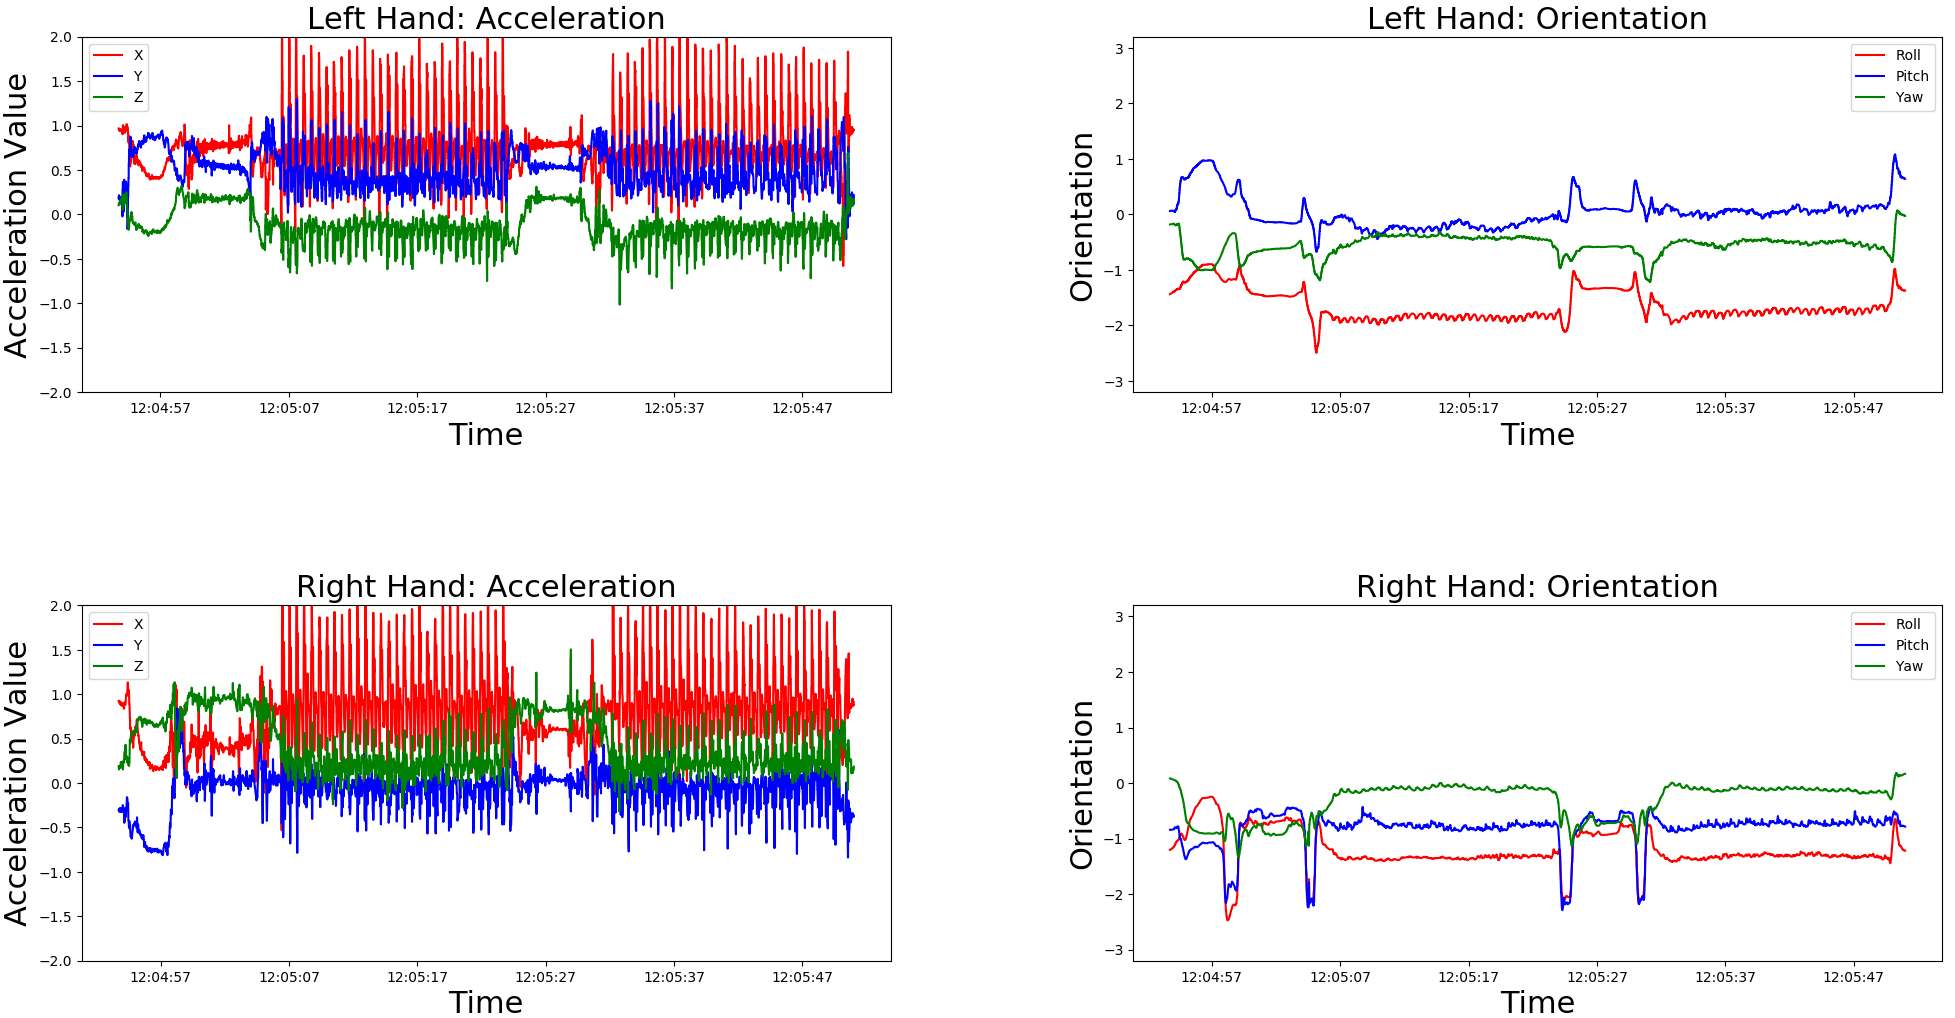
\includegraphics[width=\linewidth]{pictures/1571_IMU_Day3_cpr_31}
	\caption{IMU Data Plots for Acceleration and Orientation Data for CPR}
	\label{fig:1571imuday3cpr31}
\end{figure}
\begin{figure}[!h]
	\centering
	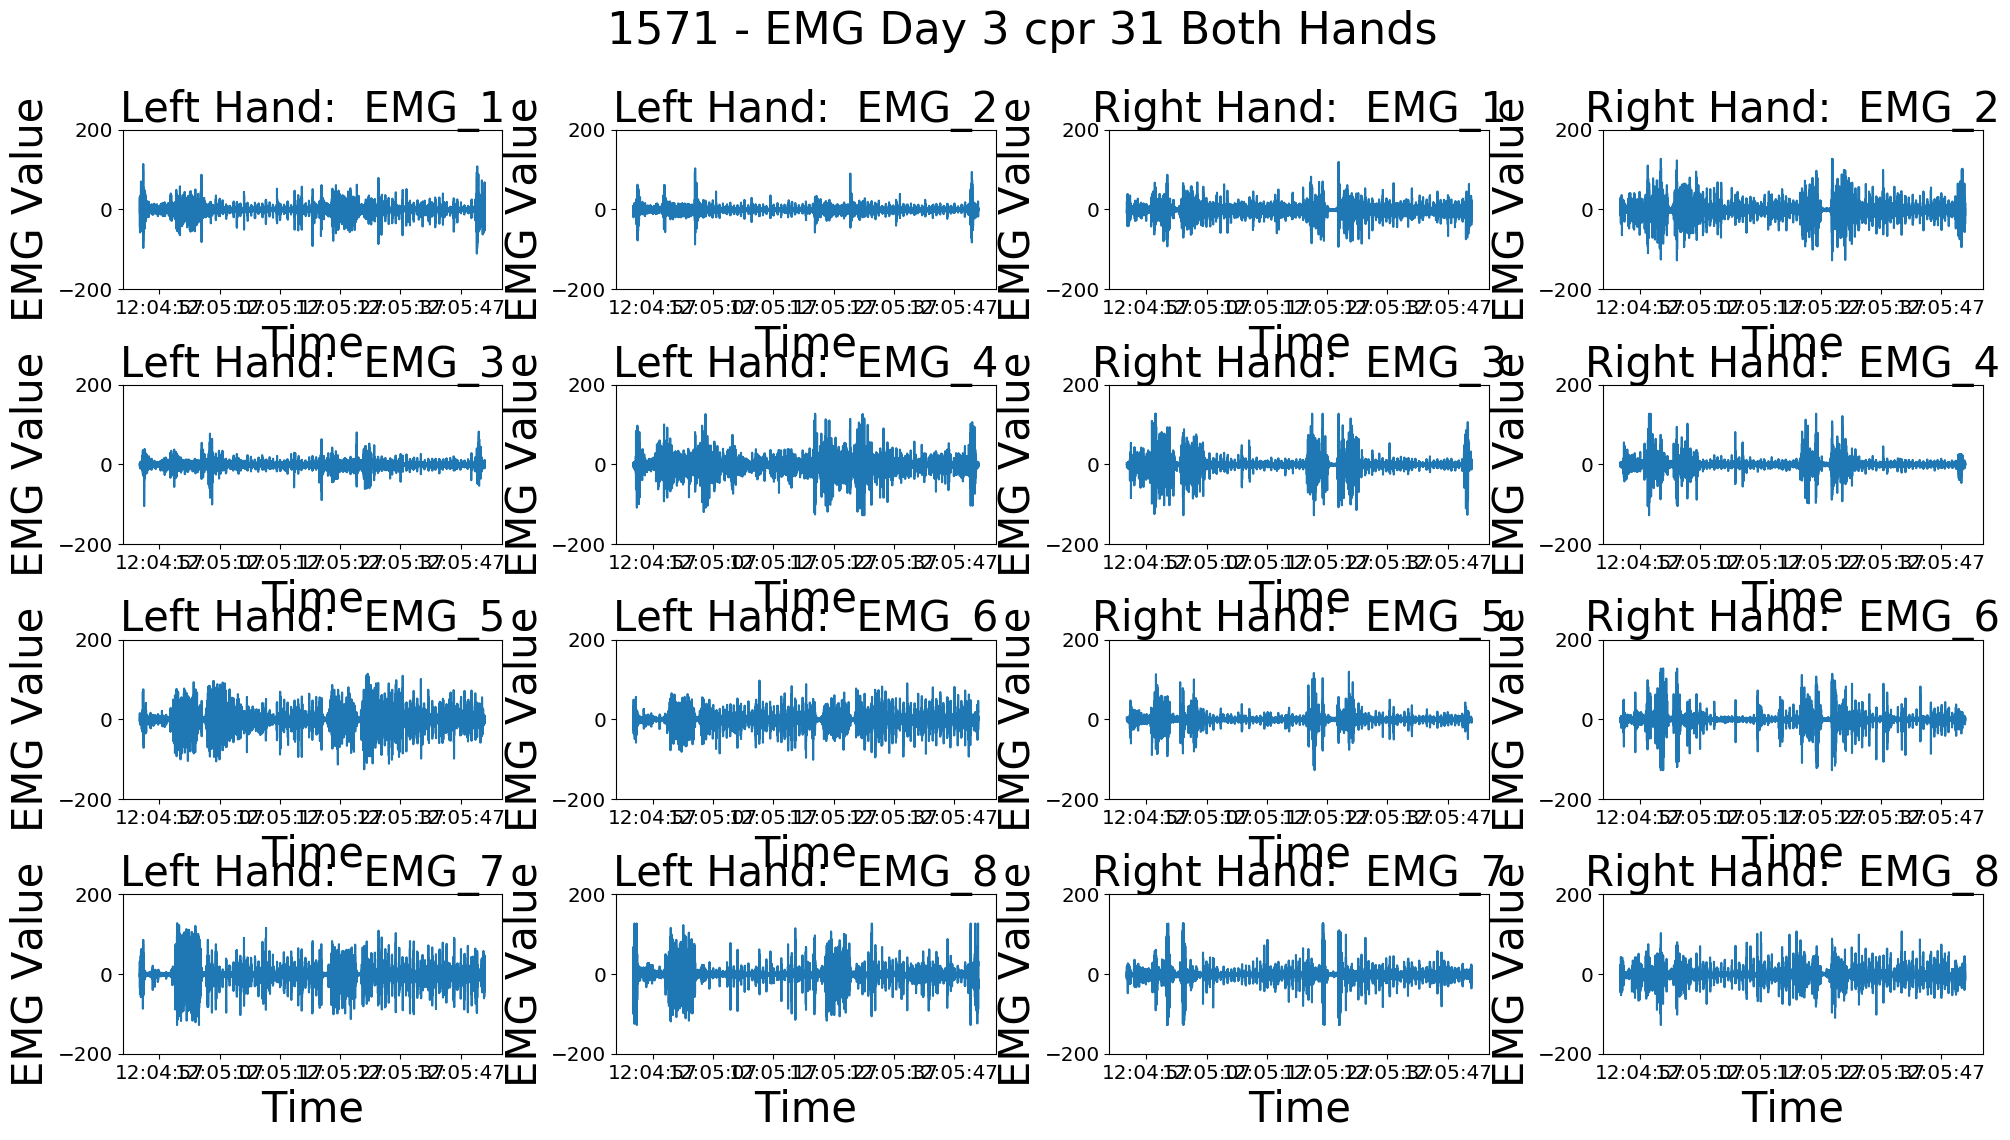
\includegraphics[width=\linewidth]{pictures/1571_EMG_Day3_cpr_31}
	\caption{EMG Data Plots for CPR}
	\label{fig:1571emgday3cpr31}
\end{figure}

Patients without adequate breathing are administered Bag-Valve-Mask ventilation. Completing one round of the Bag-Valve-Mask ventilation procedure took the participants an average of 35.39 seconds (St. Dev. = 5.70). The participants completed two rounds within one minute. The amount of instances for the third day were seven per participant, resulting in a total of 70 datasets.
\par The bag-valve-mask ventilation datasets consists of the unique squeezing the bag motion in the EMG sensor graph. The periodic motion is visible in all eight EMG channels in Figure \ref{fig:7073emgday3b46}. There was no prominent signal in the IMU data, as the right and left hands were stationary during this procedure. Figure \ref{fig:7073imuday3b46} shows almost flat lines for acceleration and orientation of both hands.
\begin{figure}[!h]
	\centering
	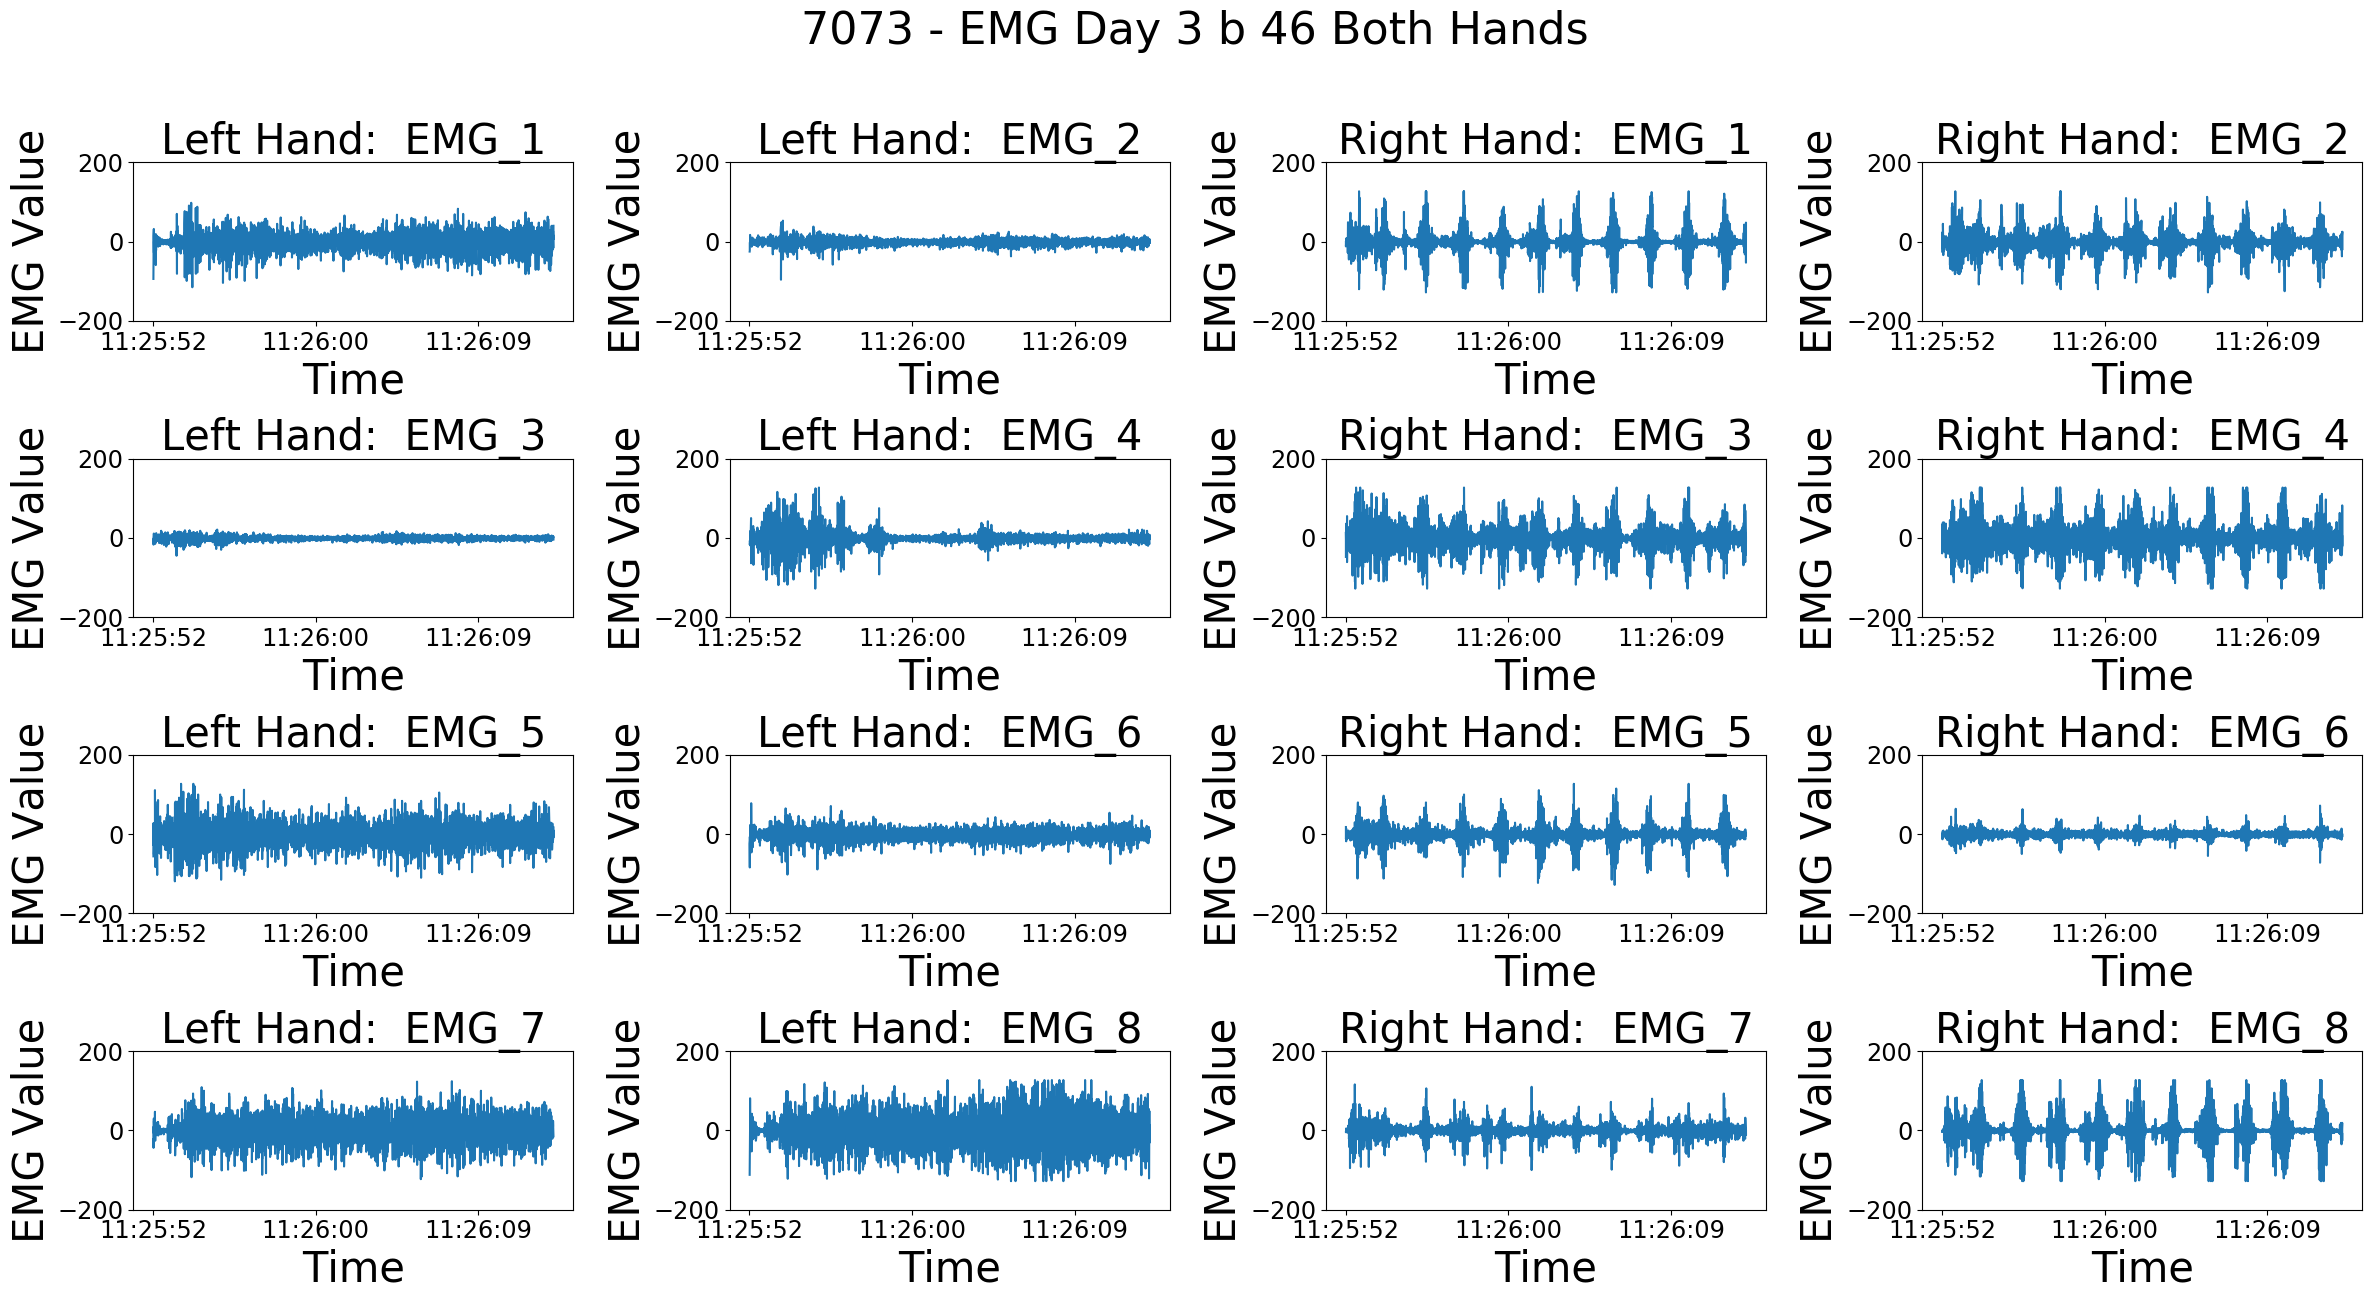
\includegraphics[width=\linewidth]{pictures/7073_EMG_Day3_b_46}
	\caption{EMG Data Plots for Bag-Valve-Mask ventilation}
	\label{fig:7073emgday3b46}
\end{figure}
\begin{figure}[!h]
	\centering
	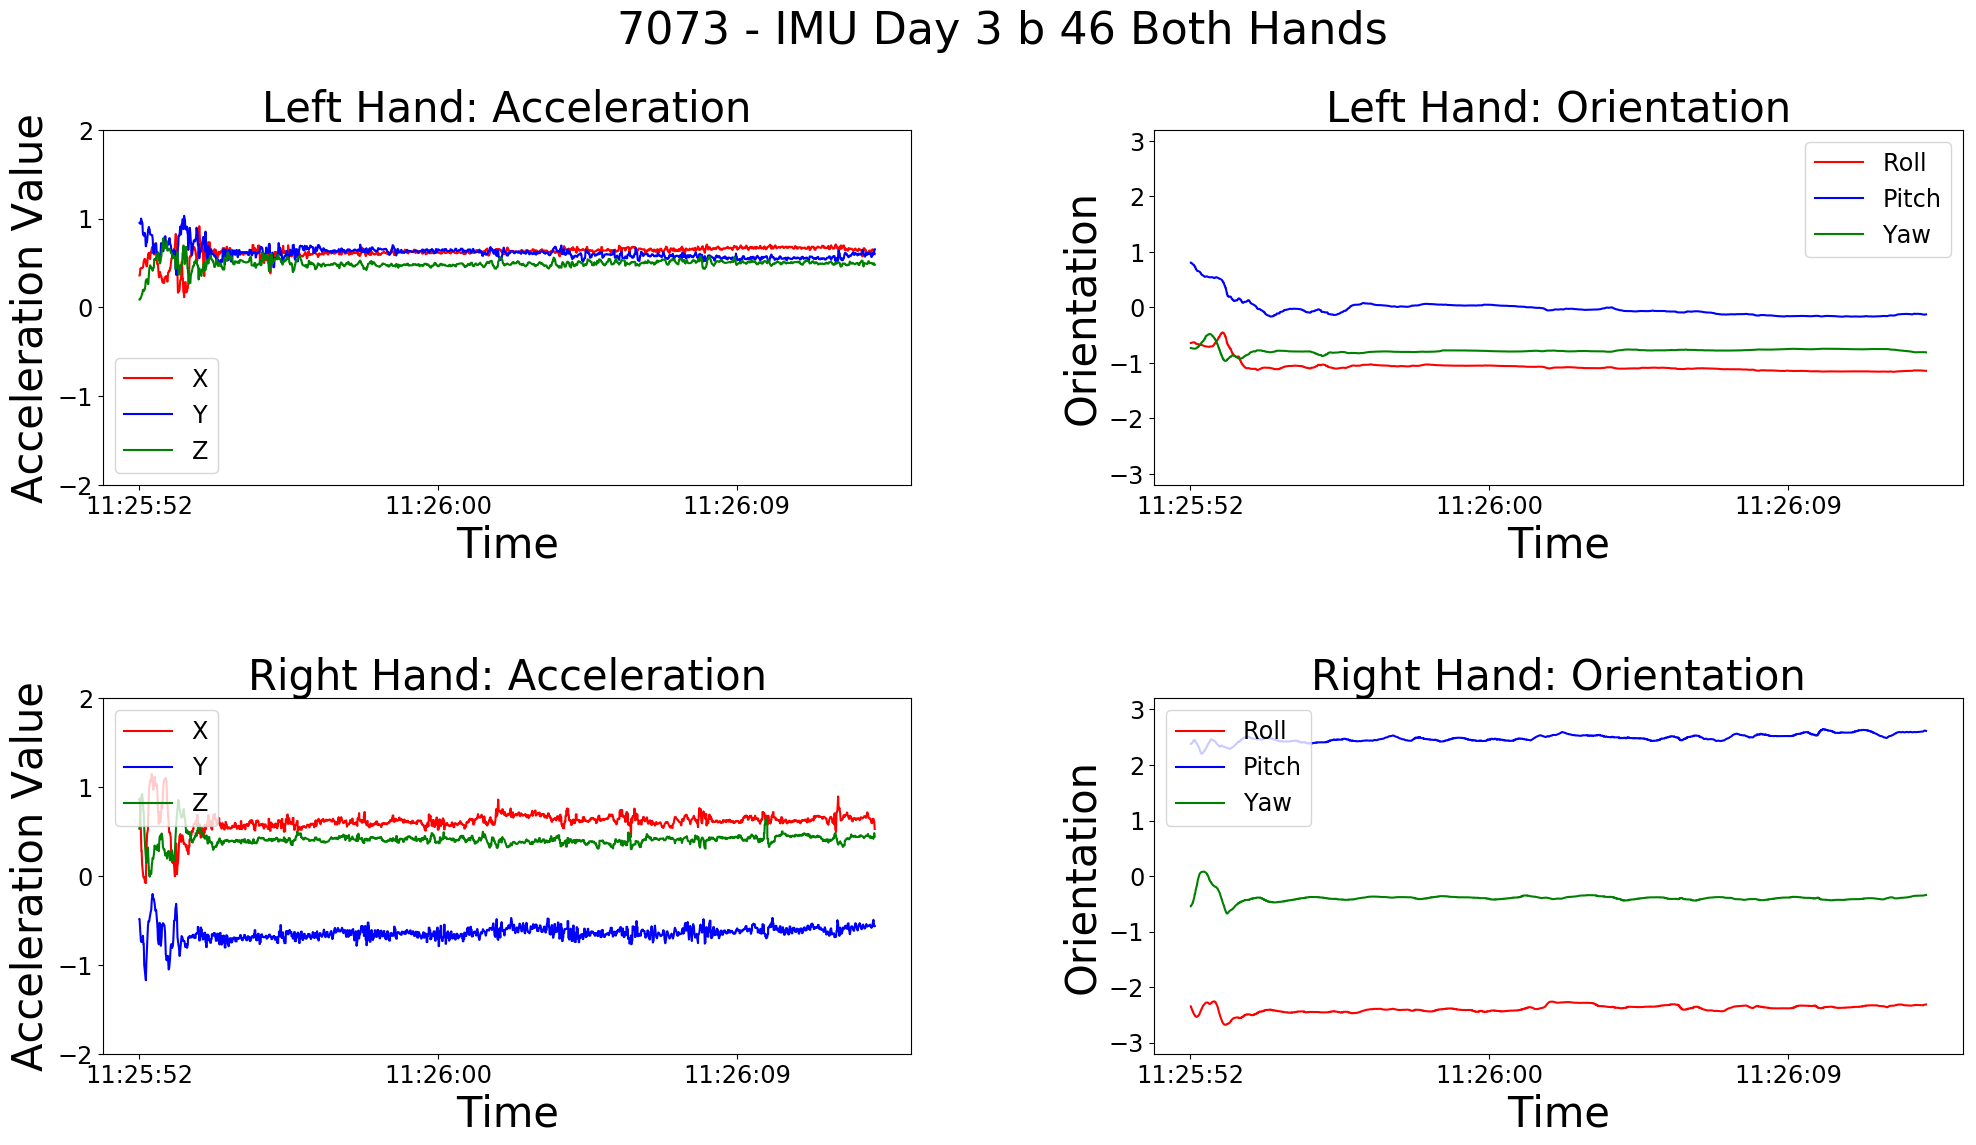
\includegraphics[width=\linewidth]{pictures/7073_IMU_Day3_b_46}
	\caption{IMU Data Plots for Acceleration and Orientation Data for Bag-Valve-Mask ventilation}
	\label{fig:7073imuday3b46}
\end{figure}

Placing an oral airway is part of the airway management procedures to prevent and relieve airway obstruction. The participants took an average of 6.51 seconds (St. Dev. = 2.23) to place an oral airway. The participants were able to complete an average of four rounds within one minute. The amount of instances for the third day were about 9 per participant, resulting in a total of about 90 instances.
\par Placing an oral airway requires the unique motion of rotating the oral airway 180 degrees after being inserted into the mouth. The rotating motion is visible in the right hand orientation graph starting at 15:14:32 with the bulge of the blue and red line in Figure \ref{fig:2334imuday3o22}. The acceleration data did not show any significant shapes of distribution. The EMG data in Figure \ref{fig:2334emgday3o22} shows a spike in channels three, four, and five when the oral airway is rotated.
\begin{figure}[!h]
	\centering
	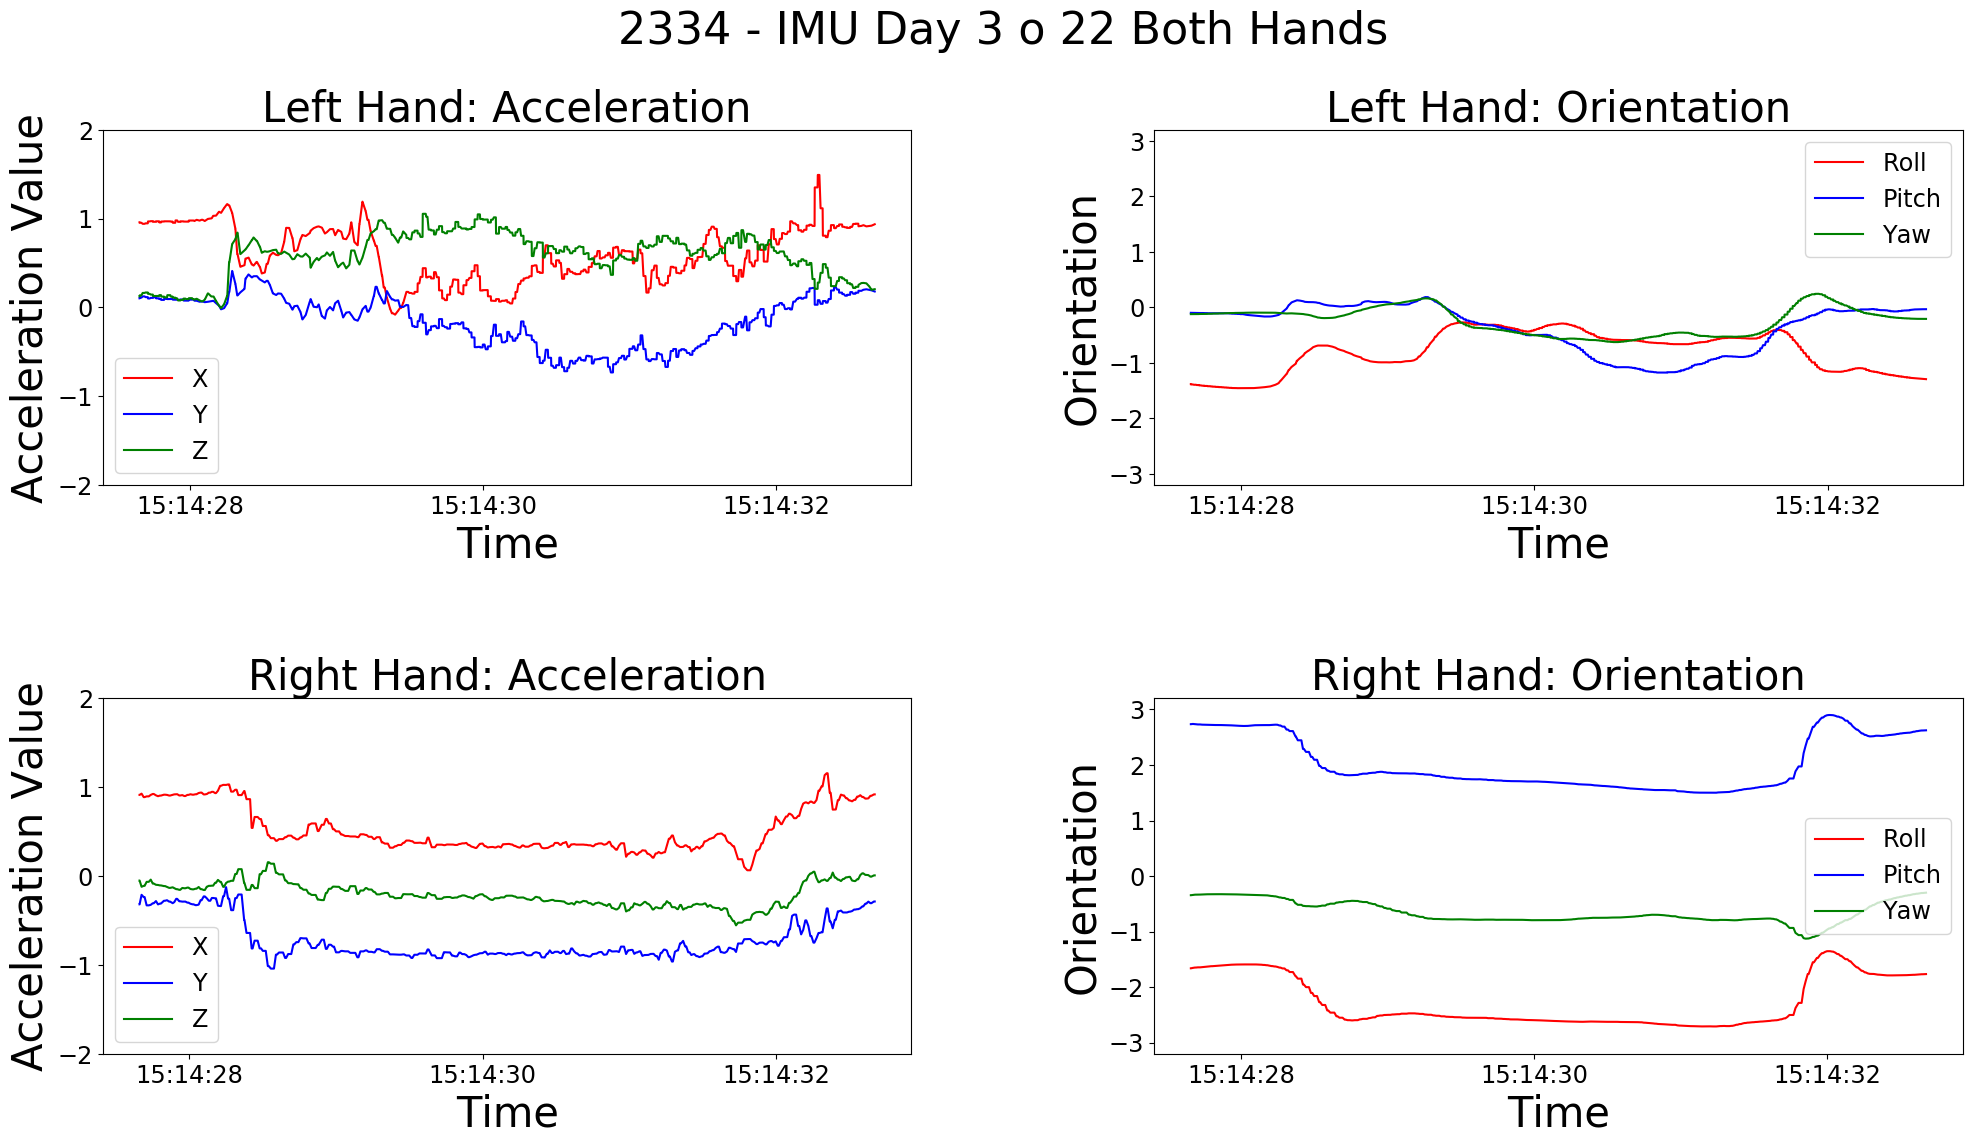
\includegraphics[width=\linewidth]{pictures/2334_IMU_Day3_o_22}
	\caption{IMU Data Plots for Acceleration and Orientation Data for Placing an Oral Airway}
	\label{fig:2334imuday3o22}
\end{figure}
\begin{figure}[!h]
	\centering
	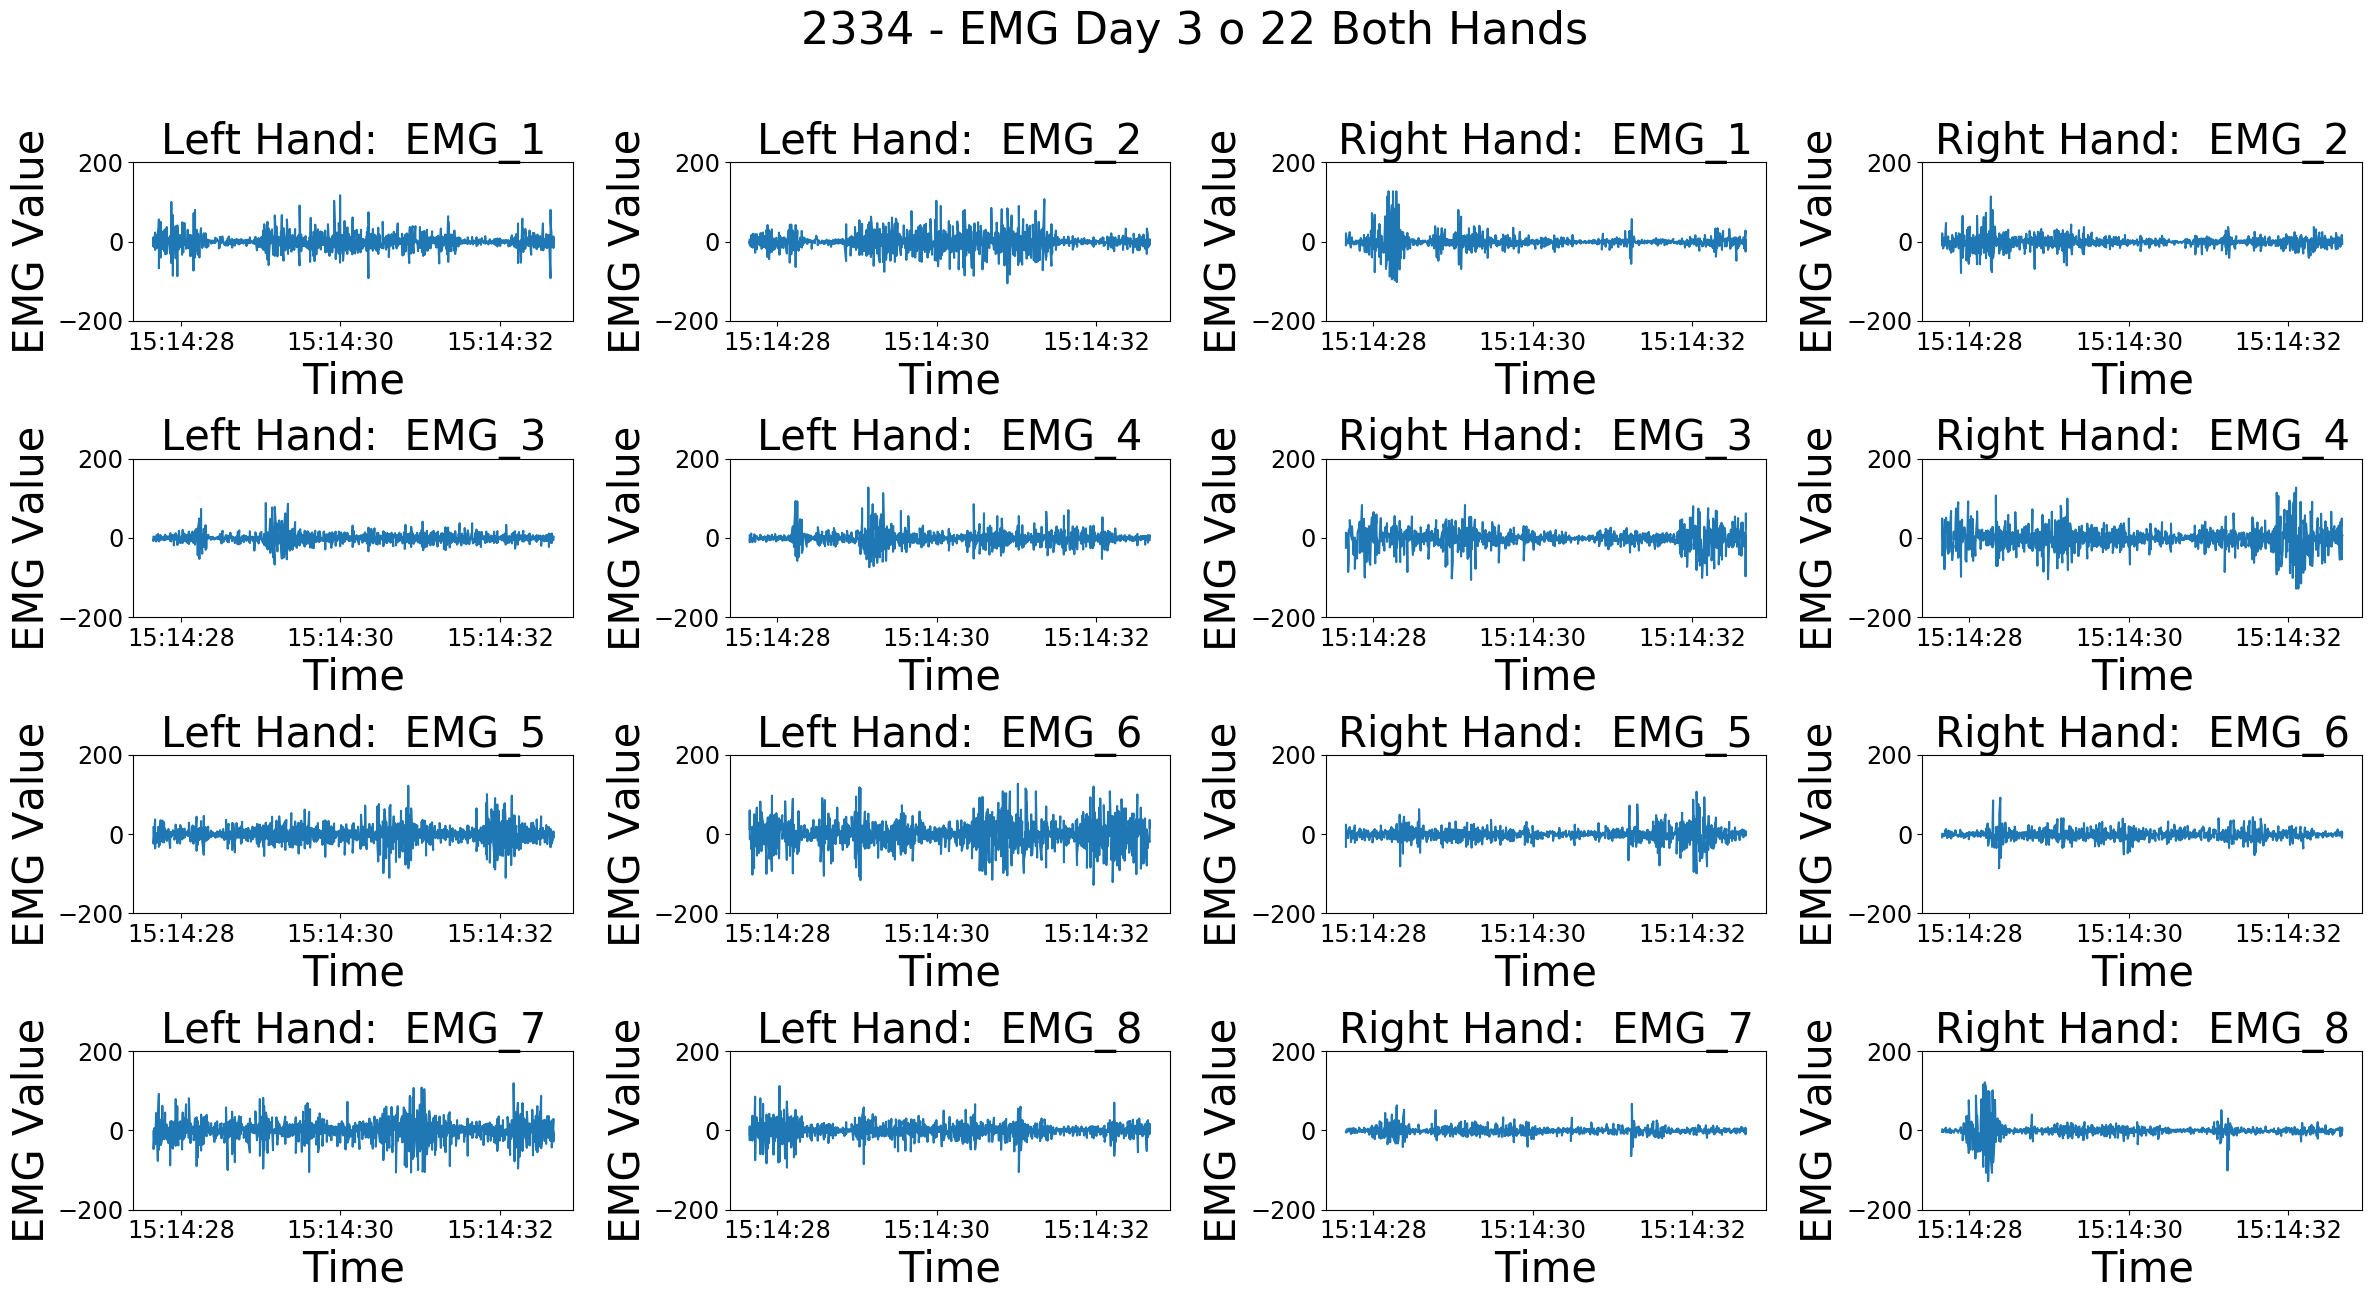
\includegraphics[width=\linewidth]{pictures/2334_EMG_Day3_o_22}
	\caption{EMG Data Plots for Placing an Oral Airway}
	\label{fig:2334emgday3o22}
\end{figure}

An intravenous tourniquet is used to restrict blood flow on a patient. The participants took an average of 9.38 seconds (St. Dev. = 2.70) to place an intravenous tourniquet. The participants were able to complete an average of three rounds within the one minute data collection of every procedure. The amount of instances for the third day were seven per participant, resulting in a total of 70 datasets.
\par The placing of an intravenous tourniquet consists of a single wrapping motion around the arm and tying of the ends. The wrapping and tying motion was visible in the IMU's orientation data starting at 9:09:09 with periodic movement and finishing at 09:09:15 with a spike in Figure \ref{fig:4501imuday3t7}. The acceleration and EMG in Figure \ref{fig:4501emgday3t7} data do not show any significant pattern.
\begin{figure}[!h]
	\centering
	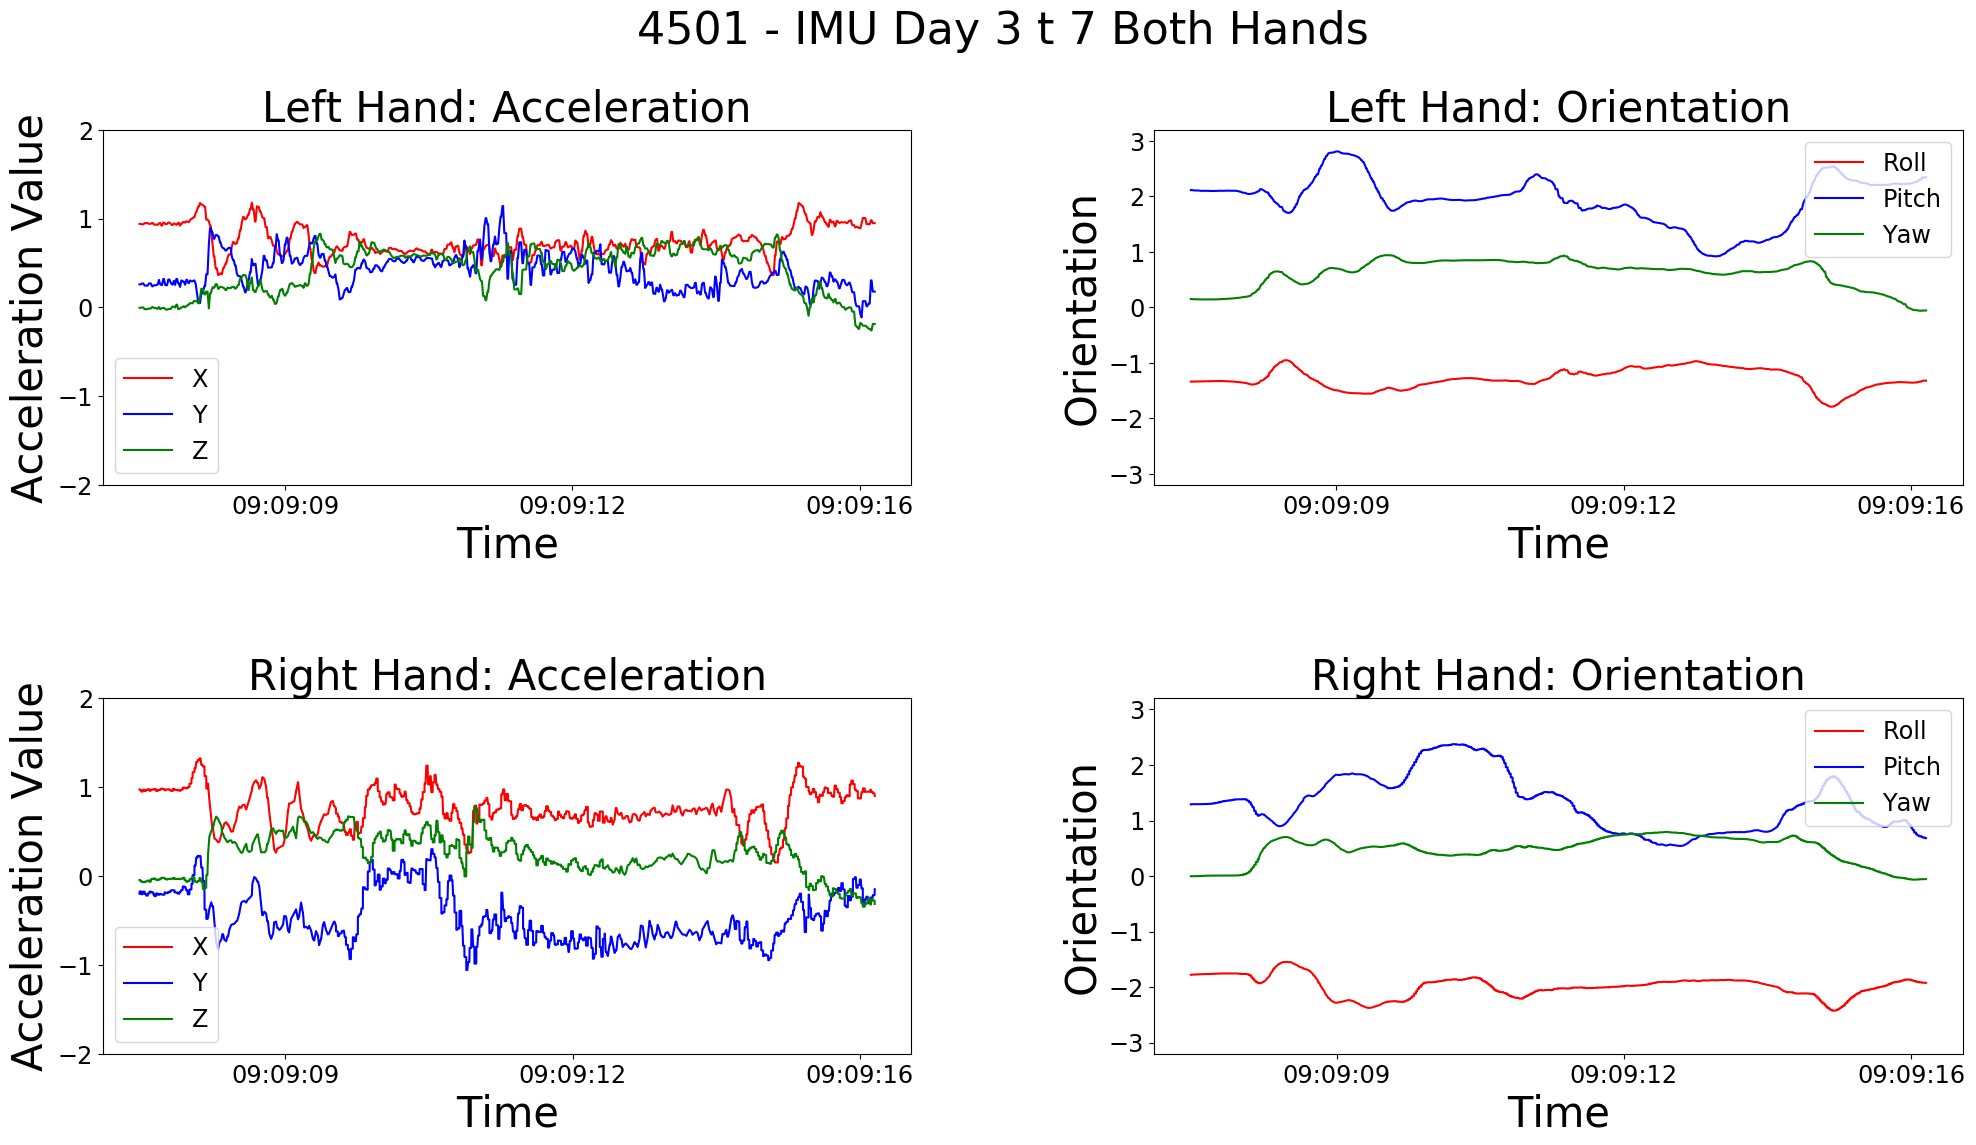
\includegraphics[width=\linewidth]{pictures/4501_IMU_Day3_t_7}
	\caption{IMU Data Plots for Acceleration and Orientation Data for Placing an IV Tourniquet}
	\label{fig:4501imuday3t7}
\end{figure}
\begin{figure}[!h]
	\centering
	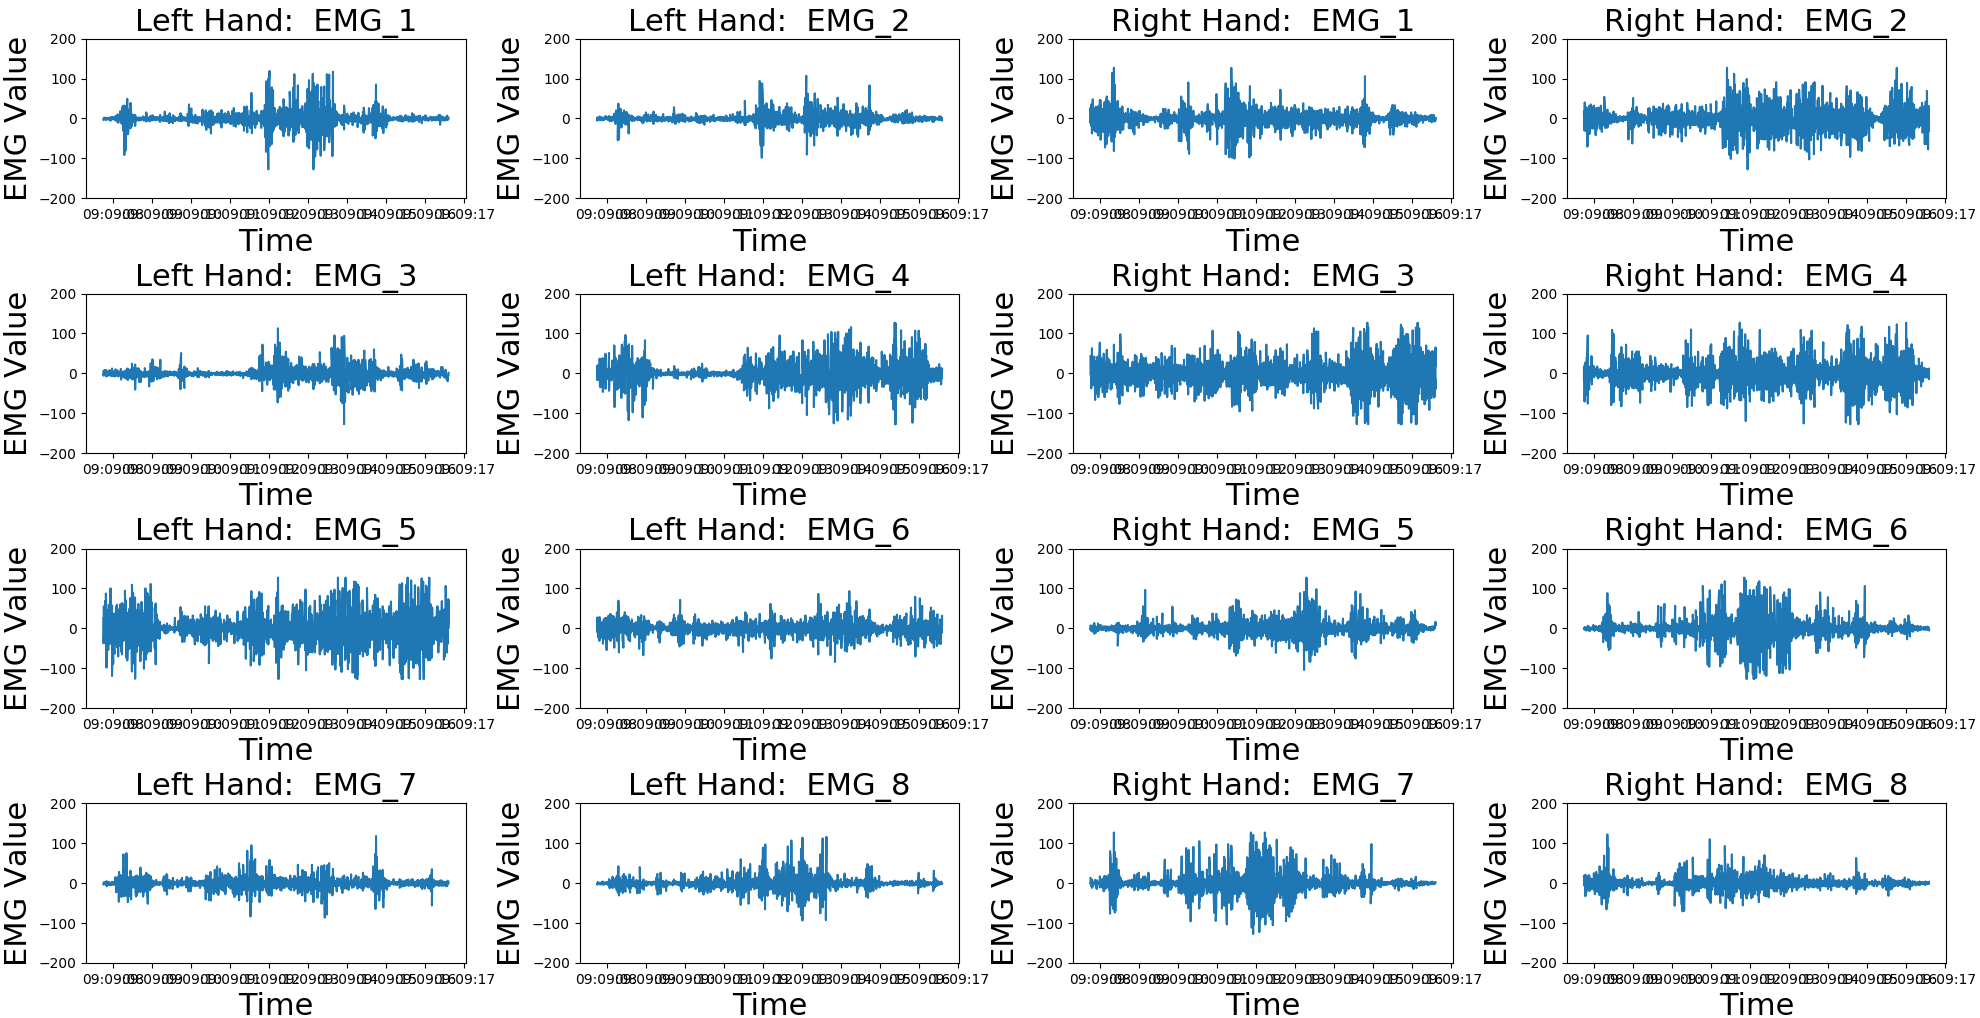
\includegraphics[width=\linewidth]{pictures/4501_EMG_Day3_t_7}
	\caption{EMG Data Plots for Placing an IV Tourniquet}
	\label{fig:4501emgday3t7}
\end{figure}

Wrapping a head wound is used to bandage a bleeding on a patient's head. Completely wrapping a head wound took participants an average of 37.26 seconds (St. Dev. = 11.72). The participants were able to complete two rounds within the one minute. The amount of instances for the third day were seven per participant, resulting in a total of 70 instances.
\par The Wrapping of a head wound consists of the unique movement of bandaging around the head of a patient. The wrapping motion is primarily visible in the orientation data of the IMU in Figure \ref{fig:2334imuday3w47}. The spikes in the orientation data at 15:27:18 are sinusoidal and represent the amount of rotations around the head. The EMG data in Figure \ref{fig:2334emgday3w47} shows a substantial amount of activity related to the grabbing and releasing of the bandage when wrapping around the patient's head.
\begin{figure}[!h]
	\centering
	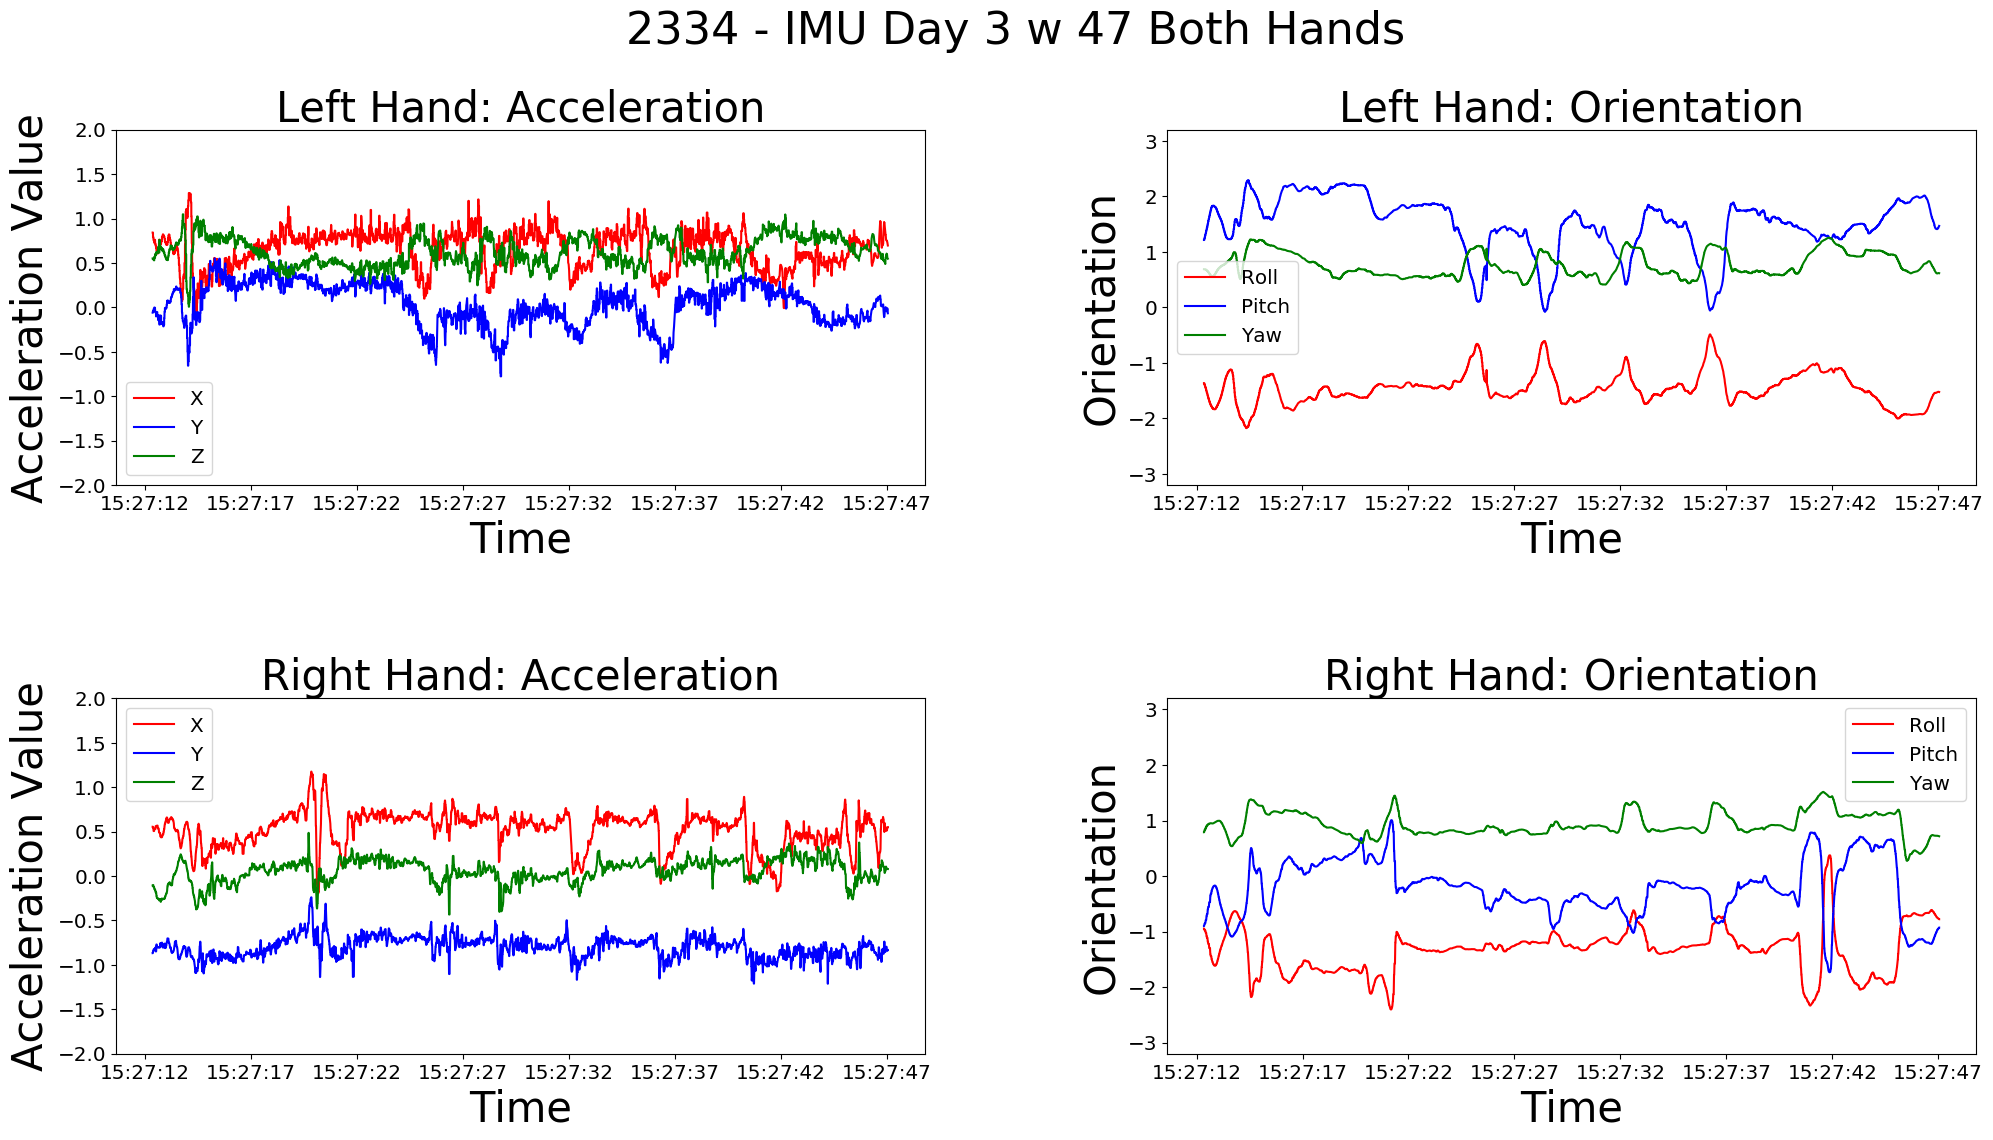
\includegraphics[width=\linewidth]{pictures/2334_IMU_Day3_w_47}
	\caption{IMU Data Plots for Acceleration and Orientation Data for wrapping a head wound}
	\label{fig:2334imuday3w47}
\end{figure}
\begin{figure}[!h]
	\centering
	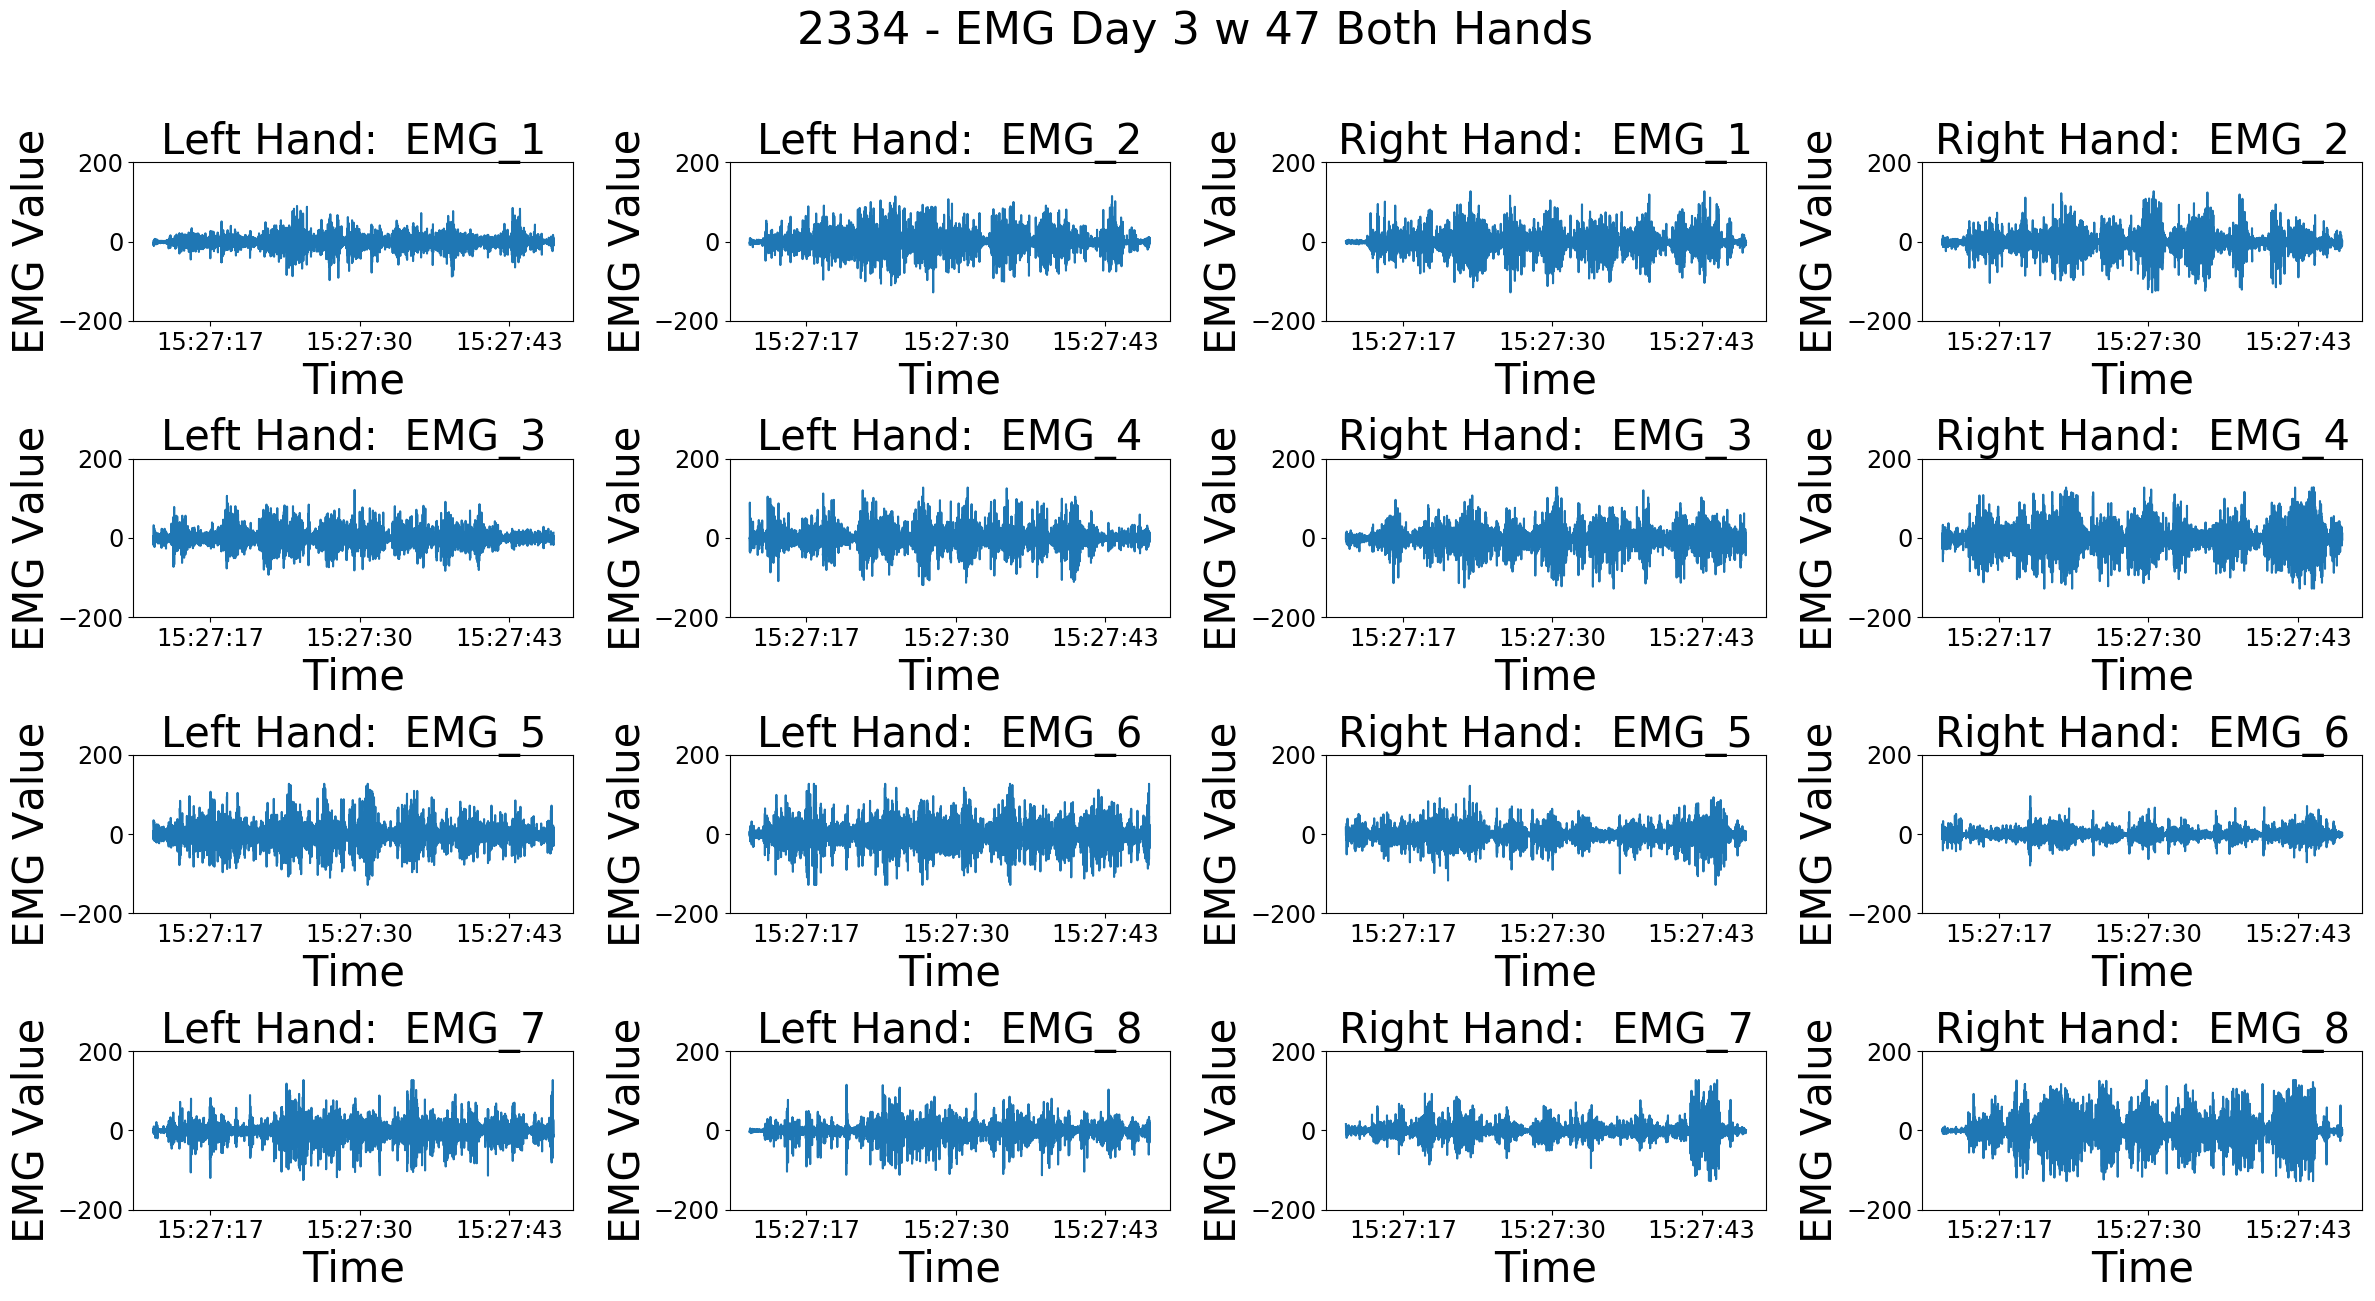
\includegraphics[width=\linewidth]{pictures/2334_EMG_Day3_w_47}
	\caption{EMG Data Plots for Wrapping a Head Wound}
	\label{fig:2334emgday3w47}
\end{figure}


\subsection{IMU and EMG Patterns Discussion}
\label{sec:Results:Patterns:Discussion}

\par The average time it takes to complete a procedure was used to detect potential outliers. Participants average time had to be within the standard deviation to be considered for the combined dataset of participant generalizability. Participant's 5 average time was outside of the overall average for all procedures and removed for the combined dataset.

\par The sinusoidal movement of the chest compressions in the acceleration data when performing the CPR procedure can make it easy for a machine learning algorithm to pick up on, due to the unique value for the signal magnitude area feature. The sequence of applying chest compressions twice during one run of the procedure can help the HMM algorithm identify CPR better, because of similar values occurring multiple times.

\par The Bag-Valve-Mask ventilation procedure has a unique movement repeatedly squeezing the bag. The repetitive motion will be clearly represented in the signal magnitude area feature as well as the standard deviation feature for the EMG data.

\par Placing a IV tourniquet and an oral airway took participants the shortest time to complete. These short procedures can make it harder for a machine learning algorithm to identify the procedure, as only few window iterations will occur during the length of the procedure.

\par The repeated wrapping motion of bandaging a head wound can help machine learning algorithm identify the procedure. The movement is clearly visible in both acceleration and orientation data of the IMU.

\par The patterns identified above can improve detection accuracy through the generated features when training machine learning algorithms with the collected data. The signal magnitude area is able to pick up periodic movement, the mean is able to generate a baseline of motion, and the standard deviation depicts the quantity of motion.


\section{Individual Participant Results}
\label{sec:Results:Individual}

Each individual participant's datasets were used to train the decision-tree, SVM, $k$-NN, and HMM machine learning algorithms. The F1, precision, and recall scores by participant for the CPR procedure are provided in Table \ref{tab:cpr:ml}. The first participant had the lowest F1 score of all machine learning algorithms with 0.69 for the decision-tree, 0.31 for $k$-NN, 0.28 for SVM, 0.00 for HMM. The HMM varied the most across participants when recognizing CPR .
\newcommand*\rotv{\multirow{2}{*}{\rotatebox[origin=c]{45}}}
\begin{table}[h]
	\centering
	\begin{tabular}{lllllllllllll}
		\multirow{2}{*}{\rotatebox[origin=c]{45}{\textbf{Participant}}} & \multicolumn{3}{c}{\textbf{decision-tree}} & \multicolumn{3}{c}{\textbf{$k$-NN} ($k=4$)} & \multicolumn{3}{c}{\textbf{SVM}} & \multicolumn{3}{c}{\textbf{HMM}} \\
		& \rot{Precision}     & \rot{Recall}    & \rot{F1}    & \rot{Precision}     & \rot{Recall}    & \rot{F1}  & \rot{Precision}     & \rot{Recall}    & \rot{F1} & \rot{Precision}     & \rot{Recall}    & \rot{F1} \\
		\textbf{1}   & \textbf{0.69} & \textbf{0.69} & \textbf{0.69} & 0.37 & 0.27 & 0.31 & 0.37 & 0.22 & 0.28 & 0.00 & 0.00 & 0.00 \\
		\textbf{2}   & \textbf{0.85} & 0.83 & 0.84 & 0.36 & 0.19 & 0.25 & 0.42 & 0.36 & 0.39 & 0.44 & 0.67 & 0.53 \\
		\textbf{3}   & \textbf{0.84} & 0.81 & 0.82 & 0.41 & 0.24 & 0.31 & 0.42 & 0.37 & 0.39 & 0.40 & 0.33 & 0.36 \\
		\textbf{4}   & 0.84 & \textbf{0.86} & 0.85 & 0.54 & 0.33 & 0.41 & 0.55 & 0.47 & 0.51 & 0.42 & 0.83 & 0.56 \\
		\textbf{5}   & 0.81 & \textbf{0.82} & \textbf{0.82} & 0.66 & 0.37 & 0.47 & 0.66 & 0.50 & 0.57 & 0.29 & 0.67 & 0.40 \\
		\textbf{6}   & 0.78 & \textbf{0.80} & 0.79 & 0.36 & 0.16 & 0.22 & 0.40 & 0.34 & 0.37 & 0.36 & 0.67 & 0.47 \\
		\textbf{7}   & 0.89 & \textbf{0.91} & 0.90 & 0.55 & 0.44 & 0.49 & 0.68 & 0.53 & 0.60 & 0.38 & 1.00 & 0.55 \\
		\textbf{8}   & 0.89 & \textbf{0.90} & 0.89 & 0.22 & 0.09 & 0.13 & 0.42 & 0.37 & 0.40 & 0.12 & 0.17 & 0.14 \\
		\textbf{9}   & \textbf{0.90} & 0.87 & 0.88 & 0.49 & 0.23 & 0.31 & 0.61 & 0.47 & 0.53 & 0.50 & 0.83 & 0.62 \\
		\textbf{10} & \textbf{0.83} & 0.77 & 0.80 & 0.50 & 0.27 & 0.35 & 0.54 & 0.45 & 0.49 & 0.50 & 0.67 & 0.57 \\
		\hline
		\textbf{Mean} & \textbf{0.83} & \textbf{0.83} & \textbf{0.83} & 0.45 & 0.26 & 0.33 & 0.51 & 0.41 & 0.45 & 0.34 & 0.58 & 0.42 \\
		\textbf{Std. Dev.} & 0.06 & 0.07 & 0.06 & 0.13 & 0.10 & 0.11 & 0.12 & 0.09 & 0.10 & 0.16 & 0.32 & 0.20
	\end{tabular}
	\caption{Ten-fold cross validation for detecting CPR per participant. Note: Bold represents the highest performance across a row}
	\label{tab:cpr:ml}
\end{table}

\par Bag-Valve-Mask ventilation achieved the lowest F1 scores of all procedures with F1 scores as low as 0.08 for participant eight using the $k$-NN algorithm, as seen in Table \ref{tab:bvm:ml}. The highest F1 score was achieved by participant ten using the HMM algorithm. The HMM algorithm also achieved the highest mean F1 score at 0.64 (Std. Dev=0.19), followed by the decision-tree algorithm at 0.60 (Std. Dev=0.09), and SVM algorithm at 0.26 (Std. Dev=0.06). The $k$-NN algorithm came last with a F1 score of 0.14 (Std. Dev=0.11).
\begin{table}[h]
	\centering
	\begin{tabular}{lllllllllllll}
		\multirow{2}{*}{\rotatebox[origin=c]{45}{\textbf{Participant}}}& \multicolumn{3}{c}{\textbf{decision-tree}} & \multicolumn{3}{c}{\textbf{$k$-NN} ($k=4$)} & \multicolumn{3}{c}{\textbf{SVM}} & \multicolumn{3}{c}{\textbf{HMM}} \\
		& \rot{Precision}     & \rot{Recall}    & \rot{F1}    & \rot{Precision}     & \rot{Recall}    & \rot{F1}  & \rot{Precision}     & \rot{Recall}    & \rot{F1} & \rot{Precision}     & \rot{Recall}    & \rot{F1} \\
		\textbf{1}   & \textbf{0.81} & 0.48 & 0.60 & 0.67 & 0.30 & 0.41 & 0.31 & 0.19 & 0.23 & 0.50 & 0.25 & 0.33 \\
		\textbf{2}   & 0.79 & 0.78 & 0.78 & 0.58 & 0.17 & 0.27 & 0.31 & 0.23 & 0.26 & 0.90 & 0.75 & \textbf{0.82} \\
		\textbf{3}   & 0.56 & 0.54 & 0.55 & 0.32 & 0.13 & 0.18 & 0.32 & 0.26 & 0.29 & \textbf{0.88} & 0.70 & 0.78 \\
		\textbf{4}   & 0.47 & 0.45 & 0.46 & 0.27 & 0.06 & 0.10 & 0.22 & 0.20 & 0.21 & \textbf{0.71} & 0.50 & 0.59 \\
		\textbf{5}   & 0.71 & 0.58 & 0.64 & 0.11 & 0.04 & 0.05 & 0.24 & 0.25 & 0.25 & \textbf{0.86} & 0.60 & 0.71 \\
		\textbf{6}   & \textbf{0.55} & 0.50 & 0.53 & 0.33 & 0.07 & 0.12 & 0.38 & 0.29 & 0.32 & 0.60 & 0.33 & 0.43 \\
		\textbf{7}   & 0.62 & 0.63 & 0.63 & 0.28 & 0.07 & 0.12 & 0.26 & 0.24 & 0.25 & \textbf{1.00} & 0.57 & 0.73 \\
		\textbf{8}   & 0.50 & \textbf{0.52} & 0.51 & 0.18 & 0.05 & 0.08 & 0.16 & 0.14 & 0.15 & 0.57 & 0.44 & 0.50 \\
		\textbf{9}   & \textbf{0.63} & 0.59 & 0.61 & 0.33 & 0.09 & 0.14 & 0.33 & 0.35 & 0.34 & 0.80 & 0.44 & 0.57 \\
		\textbf{10} & 0.67 & 0.63 & 0.65 & 0.12 & 0.02 & 0.03 & 0.30 & 0.33 & 0.32 & \textbf{1.00} & 0.90 & 0.95 \\
		\hline
		\textbf{Mean} & 0.63 & 0.57 & 0.60 & 0.31 & 0.10 & 0.14 & 0.28 & 0.25 & 0.26 & \textbf{0.78} & 0.55 & 0.64 \\
		\textbf{Std. Dev.} & 0.12 & 0.01 & 0.09 & 0.17 & 0.08 & 0.11 & 0.07 & 0.06 & 0.06 & 0.18 & 0.20 & 0.19
	\end{tabular}
	\caption{Ten-fold cross validation for detecting BVM ventilation per participant}
	\label{tab:bvm:ml}
\end{table}

\par Placing an oral airway was the most difficult procedure to detect, with F1 scores as low as 0.00 for participant five using $k$-NN, as seen in Table \ref{tab:o:ml}. The highest F1 score was achieved by participant four using the HMM algorithm. The decision-tree classifier was the algorithm with the highest mean F1 score at 0.63 (Std. Dev=0.08), followed by the HMM algorithm at 0.51 (Std. Dev=0.27), and SVM algorithm at 0.20 (Std. Dev=0.04). The $k$-NN algorithm came last with a F1 score of 0.12 (Std. Dev=0.08).
\begin{table}[h]
	\centering
	\begin{tabular}{lllllllllllll}
		\multirow{2}{*}{\rotatebox[origin=c]{45}{\textbf{Participant}}} & \multicolumn{3}{c}{\textbf{decision-tree}} & \multicolumn{3}{c}{\textbf{$k$-NN} ($k=4$)} & \multicolumn{3}{c}{\textbf{SVM}} & \multicolumn{3}{c}{\textbf{HMM}} \\
		& \rot{Precision}     & \rot{Recall}    & \rot{F1}    & \rot{Precision}     & \rot{Recall}    & \rot{F1}  & \rot{Precision}     & \rot{Recall}    & \rot{F1} & \rot{Precision}     & \rot{Recall}    & \rot{F1} \\
		\textbf{1}   & 0.47 & \textbf{0.58} & 0.52 & 0.26 & 0.14 & 0.18 & 0.24 & 0.18 & 0.21 & 0.00 & 0.00 & 0.00 \\
		\textbf{2}   & 0.63 & 0.56 & 0.59 & 0.29 & 0.10 & 0.15 & 0.19 & 0.21 & 0.20 & \textbf{1.00} & 0.50 & 0.67 \\
		\textbf{3}   & 0.67 & 0.76 & 0.71 & 0.50 & 0.17 & 0.25 & 0.29 & 0.24 & 0.26 & \textbf{0.78} & 0.70 & 0.74 \\
		\textbf{4}   & 0.68 & 0.65 & 0.66 & 0.44 & 0.10 & 0.17 & 0.26 & 0.21 & 0.23 & \textbf{0.86} & 0.67 & 0.75 \\
		\textbf{5}   & \textbf{0.66} & \textbf{0.66} & \textbf{0.66} & 0.00 & 0.00 & 0.00 & 0.29 & 0.17 & 0.22 & 0.62 & 0.56 & 0.59 \\
		\textbf{6}   & 0.71 & 0.71 & 0.71 & 0.27 & 0.06 & 0.10 & 0.16 & 0.15 & 0.16 & \textbf{0.75} & 0.67 & 0.71 \\
		\textbf{7}   & \textbf{0.60} & 0.59 & \textbf{0.60} & 0.12 & 0.03 & 0.05 & 0.23 & 0.18 & 0.20 & 0.50 & 0.14 & 0.22 \\
		\textbf{8}   & 0.71 & \textbf{0.78} & 0.74 & 0.38 & 0.12 & 0.19 & 0.28 & 0.20 & 0.23 & 0.25 & 0.11 & 0.15 \\
		\textbf{9}   & 0.62 & 0.66 & 0.64 & 0.09 & 0.04 & 0.05 & 0.15 & 0.11 & 0.13 & \textbf{0.80} & 0.50 & 0.62 \\
		\textbf{10} & 0.54 & 0.59 & 0.57 & 0.40 & 0.06 & 0.10 & 0.16 & 0.13 & 0.14 & \textbf{0.67} & 0.57 & 0.62 \\
		\hline
		\textbf{Mean} & 0.63 & \textbf{0.65} & 0.63 & 0.28 & 0.08 & 0.12 & 0.22 & 0.18 & 0.20 & 0.62 & 0.44 & 0.51 \\
		\textbf{Std. Dev.} & 0.08 & 0.08 & 0.08 & 0.16 & 0.05 & 0.08 & 0.06 & 0.04 & 0.04 & 0.30 & 0.26 & 0.27 \\
	\end{tabular}
	\caption{Ten-fold cross validation for detecting oral airway placement per participant}
	\label{tab:o:ml}
\end{table}

\par Placing an IV tourniquet achieved a good F1 score for all machine learning algorithms except the HMM algorithm, as seen in Table \ref{tab:t:ml}. The lowest F1 score of 0.00 were achieved by participants two, three, and five. The highest F1 score was 0.87 by participant eight using the decision-tree. The decision-tree classifier was the algorithm with the highest mean F1 score at 0.81 (Std. Dev=0.06), followed by the SVM algorithm at 0.53 (Std. Dev=0.10), and $k$-NN at 0.40 (Std. Dev=0.05). The HMM algorithm came last with a F1 score of 0.24 (Std. Dev=0.21).
\begin{table}[h]
	\centering
	\begin{tabular}{lllllllllllll}
		\multirow{2}{*}{\rotatebox[origin=c]{45}{\textbf{Participant}}} & \multicolumn{3}{c}{\textbf{decision-tree}} & \multicolumn{3}{c}{\textbf{$k$-NN} ($k=4$)} & \multicolumn{3}{c}{\textbf{SVM}} & \multicolumn{3}{c}{\textbf{HMM}} \\
		& \rot{Precision}     & \rot{Recall}    & \rot{F1}    & \rot{Precision}     & \rot{Recall}    & \rot{F1}  & \rot{Precision}     & \rot{Recall}    & \rot{F1} & \rot{Precision}     & \rot{Recall}    & \rot{F1} \\
		\textbf{1}   & \textbf{0.65} & \textbf{0.65} & \textbf{0.65} & 0.30 & 0.36 & 0.33 & 0.29 & 0.30 & 0.30 & 0.22 & 0.40 & 0.29 \\
		\textbf{2}   & 0.80 & \textbf{0.81} & 0.80 & 0.31 & 0.56 & 0.40 & 0.51 & 0.62 & 0.56 & 0.00 & 0.00 & 0.00 \\
		\textbf{3}   & \textbf{0.83} & 0.81 & 0.82 & 0.30 & 0.57 & 0.39 & 0.43 & 0.56 & 0.49 & 0.00 & 0.00 & 0.00 \\
		\textbf{4}   & 0.84 & \textbf{0.85} & 0.84 & 0.37 & 0.64 & 0.47 & 0.56 & 0.67 & 0.61 & 0.50 & 0.17 & 0.25 \\
		\textbf{5}   & 0.85 & \textbf{0.87} & 0.86 & 0.34 & 0.64 & 0.45 & 0.54 & 0.71 & 0.61 & 0.00 & 0.00 & 0.00 \\
		\textbf{6}   & \textbf{0.83} & 0.80 & 0.82 & 0.31 & 0.42 & 0.36 & 0.48 & 0.59 & 0.53 & 0.33 & 0.17 & 0.22 \\
		\textbf{7}   & \textbf{0.80} & 0.79 & \textbf{0.80} & 0.27 & 0.44 & 0.33 & 0.42 & 0.55 & 0.48 & 0.22 & 0.33 & 0.27 \\
		\textbf{8}   & \textbf{0.89} & 0.86 & 0.87 & 0.33 & 0.60 & 0.43 & 0.50 & 0.66 & 0.57 & 0.60 & 0.50 & 0.55 \\
		\textbf{9}   & \textbf{0.80} & 0.78 & 0.79 & 0.34 & 0.53 & 0.41 & 0.47 & 0.59 & 0.53 & 0.75 & 0.50 & 0.60 \\
		\textbf{10} & 0.80 & \textbf{0.84} & 0.82 & 0.28 & 0.52 & 0.37 & 0.43 & 0.53 & 0.58 & 0.25 & 0.17 & 0.20 \\
		\hline
		\textbf{Mean} & \textbf{0.81} & \textbf{0.81} & \textbf{0.81} & 0.32 & 0.52 & 0.40 & 0.46 & 0.60 & 0.53 & 0.30 & 0.22 & 0.24 \\
		\textbf{Std. Dev.} & 0.06 & 0.06 & 0.06 & 0.03 & 0.10 & 0.05 & 0.08 & 0.11 & 0.10 & 0.26 & 0.20 & 0.21
	\end{tabular}
	\caption{Ten-fold cross validation for detecting tourniquet placement per participant}
	\label{tab:t:ml}
\end{table}

\par Wrapping a head wound achieved the highest F1 for the decision-tree algorithm of 0.93 for participants eight and ten, as seen in Table \ref{tab:w:ml}. The lowest F1 score was 0.00 for participant seven using the HMM algorithm. The decision-tree classifier had a mean F1 score of 0.90 (Std. Dev=0.06), followed by the SVM algorithm at 0.61 (Std. Dev=0.04), and $k$-NN at 0.50 (Std. Dev=0.04). The HMM algorithm came last with a F1 score of 0.40 (Std. Dev=0.18)
\begin{table}[]
	\centering
	\begin{tabular}{lllllllllllll}
		\multirow{2}{*}{\rotatebox[origin=c]{45}{\textbf{Participant}}} & \multicolumn{3}{c}{\textbf{decision-tree}} & \multicolumn{3}{c}{\textbf{$k$-NN} ($k=4$)} & \multicolumn{3}{c}{\textbf{SVM}} & \multicolumn{3}{c}{\textbf{HMM}} \\
		& \rot{Precision}     & \rot{Recall}    & \rot{F1}    & \rot{Precision}     & \rot{Recall}    & \rot{F1}  & \rot{Precision}     & \rot{Recall}    & \rot{F1} & \rot{Precision}     & \rot{Recall}    & \rot{F1} \\
		\textbf{1}   & \textbf{0.73} & 0.72 & 0.72 & 0.43 & 0.54 & 0.48 & 0.47 & 0.66 & 0.55 & 0.20 & 0.20 & 0.20 \\
		\textbf{2}   & 0.88 & \textbf{0.91} & 0.89 & 0.45 & 0.46 & 0.46 & 0.60 & 0.58 & 0.59 & 0.30 & 0.50 & 0.37 \\
		\textbf{3}   & 0.81 & \textbf{0.83} & 0.82 & 0.42 & 0.42 & 0.42 & 0.63 & 0.62 & 0.62 & 0.38 & 0.83 & 0.53 \\
		\textbf{4}   & \textbf{0.91} & 0.90 & 0.90 & 0.43 & 0.49 & 0.46 & 0.61 & 0.63 & 0.62 & 0.22 & 0.33 & 0.27 \\
		\textbf{5}   & \textbf{0.87} & \textbf{0.87} & \textbf{0.87} & 0.42 & 0.39 & 0.40 & 0.63 & 0.63 & 0.63 & 0.29 & 0.33 & 0.31 \\
		\textbf{6}   & 0.88 & \textbf{0.90} & 0.89 & 0.45 & 0.65 & 0.53 & 0.54 & 0.55 & 0.55 & 0.44 & 0.67 & 0.53 \\
		\textbf{7}   & \textbf{0.92} & 0.91 & \textbf{0.92} & 0.49 & 0.54 & 0.51 & 0.60 & 0.65 & 0.62 & 0.00 & 0.00 & 0.00 \\
		\textbf{8}   & \textbf{0.94} & 0.92 & 0.93 & 0.43 & 0.48 & 0.45 & 0.62 & 0.59 & 0.61 & 0.25 & 0.50 & 0.33 \\
		\textbf{9}   & 0.88 & \textbf{0.90} & 0.89 & 0.49 & 0.55 & 0.51 & 0.68 & 0.68 & 0.68 & 0.45 & 0.83 & 0.59 \\
		\textbf{10} & 0.92 & \textbf{0.93} & \textbf{0.93} & 0.44 & 0.51 & 0.47 & 0.66 & 0.67 & 0.67 & 0.38 & 0.50 & 0.43 \\
		\hline
		\textbf{Mean} & \textbf{0.90} & \textbf{0.90} & \textbf{0.90} & 0.44 & 0.50 & 0.50 & 0.60 & 0.63 & 0.61 & 0.30 & 0.50 & 0.40 \\
		\textbf{Std. Dev.} & 0.06 & 0.06 & 0.06 & 0.03 & 0.07 & 0.04 & 0.06 & 0.04 & 0.04 & 0.13 & 0.30 & 0.18
	\end{tabular}
	\caption{Ten-fold cross validation for detecting wrapping a wound per participant}
	\label{tab:w:ml}
\end{table}

\subsection{Individual Participant Results Discussion}
\label{sec:Results:Individual:Discussion}
Contrary to the initial assumption in $H_1$, recognition of CPR and Bag-valve-mask ventilation will have the highest accuracy for each machine learning algorithm, due to its unique movements, the unique movements during CPR were not as helpful to accurately detect the procedure. The hypothesis was not supported. The overlap of the giving breaths motion resulted in CPR being misclassified as Bag-Valve-Mask ventilation. Segmenting out the chest-compressions from the breathing motions and only training using the chest-compressions may result in higher accuracy due to the chest-compressions not appearing in any other procedure.
\par Results between the participants varied greatly. The HMM algorithm scored 0.61 for one participant and 0.00 for another participant, see Table \ref{tab:cpr:ml}. Other algorithms, such as decision-tree and SVM were more stable as indicated by a low standard deviation.
\par The Bag-Valve-Mask ventilation procedure has such a unique squeezing movement that the initial assumption concluded that it will be one of the easiest procedures to detect. In contrast it turned out to be one of the hardest, which may be due to its movement overlap with CPR.
\par The F1 scores show that detecting the placement of an oral airway is challenging. The short duration for the placemet does not leave much time for the algorithm to detect unique movements. The grabbing and spinning motion can occur in several other procedures when equipment are picked up and put into place.
\par The low score of the HMM algorithm for placing an intravenous tourniquet can be a result of a close log probability of the HMM models. The HMM algorithm picks the highest log probability when data is tested on all HMM models. If the log probability are close it can mean the motion is easily interchangeable.
\par The HMM algorithm for wrapping a head wound under performed at detecting the procedure and had the highest standard deviation across participants. Participant seven achieved 0.92 for the decision-tree algorithm, but 0.00 for the HMM algorithm. The wide gap between recognition scores can contribute to the problem the HMM algorithm has with selecting the best model given the log probabilities.

\section{Participant Generalizability}
\label{sec:Results:Generalizability}

The datasets of all participants is combined to create one large dataset. The F1 score in Table \ref{tab:ml} is lower when comparing the machine learning algorithms on the combined dataset to the individual participants, Tables \ref{tab:cpr:ml} through \ref{tab:w:ml}. The highest F1 score on the combined dataset is achieved by the decision-tree algorithm with 0.71. The HMM algorithm followed second with 0.44, then $k$-NN with 0.35, and last the SVM with 0.25. Wrapping a wound (W) was the procedure with the highest F1 score for the decision-tree, $k$-NN ($k=4$) and SVM algorithm. Bag-Valve-Mask ventilation (B) was the procedure with the highest F1 score for the HMM algorithm.
\begin{table}[!h]
	\centering
	\begin{tabular}{lllllllllllll}
		\multirow{2}{*}{\rotatebox[origin=c]{45}{\textbf{Procedure}}} & \multicolumn{3}{c}{\textbf{decision-tree}} & \multicolumn{3}{c}{\textbf{$k$-NN} ($k=4$)} & \multicolumn{3}{c}{\textbf{SVM}} & \multicolumn{3}{c}{\textbf{HMM}} \\
		 & \rot{Precision}     & \rot{Recall}    & \rot{F1}    & \rot{Precision}     & \rot{Recall}    & \rot{F1}  & \rot{Precision}     & \rot{Recall}    & \rot{F1} & \rot{Precision}     & \rot{Recall}    & \rot{F1} \\
		 T & 0.73 & 0.74 & 0.74 & 0.33 & 0.56 & 0.41 & 0.53 & 0.62 & 0.57 & 0.29 & 0.36 & 0.32 \\
		 W & 0.82 & 0.82 & 0.82 & 0.42 & 0.45 & 0.43 & 0.57 & 0.72 & 0.64 & 0.19 & 0.20 & 0.20 \\
		 B & 0.39 & 0.38 & 0.39 & 0.24 & 0.07 & 0.11 & 0.18 & 0.10 & 0.13 & 0.69 & 0.71 & 0.70 \\
		 O & 0.48 & 0.46 & 0.47 & 0.23 & 0.06 & 0.10 & 0.25 & 0.13 & 0.17 & 0.60 & 0.33 & 0.43 \\
		 C & 0.69 & 0.69 & 0.69 & 0.42 & 0.27 & 0.33 & 0.48 & 0.35 & 0.41 & 0.39 & 0.50 & 0.44 \\
		 \hline
		 All & 0.71 & 0.71 & 0.71 & 0.37 & 0.37 & 0.35 & 0.49 & 0.52 & 0.49 & 0.47 & 0.44 & 0.44 \\
	\end{tabular}
	\caption{Ten-fold cross validation for all participants by procedure and algorithm. Note: T is intravenous tourniquet, W is wrapping a wound, B is Bag-Valve-Mask ventilation, O is oral airway, and C is CPR}
	\label{tab:ml}
\end{table}
The differences in movement between participants can be seen in Figure \ref{fig:5187emgday3t1average}. The Figure shows the average of placing an intravenous tourniquet for all participants in red. Similarities between the average EMG data and the data of the participant can be seen, yet some noise is observable in channels three, four, and five.
\begin{figure}[!h]
	\centering
	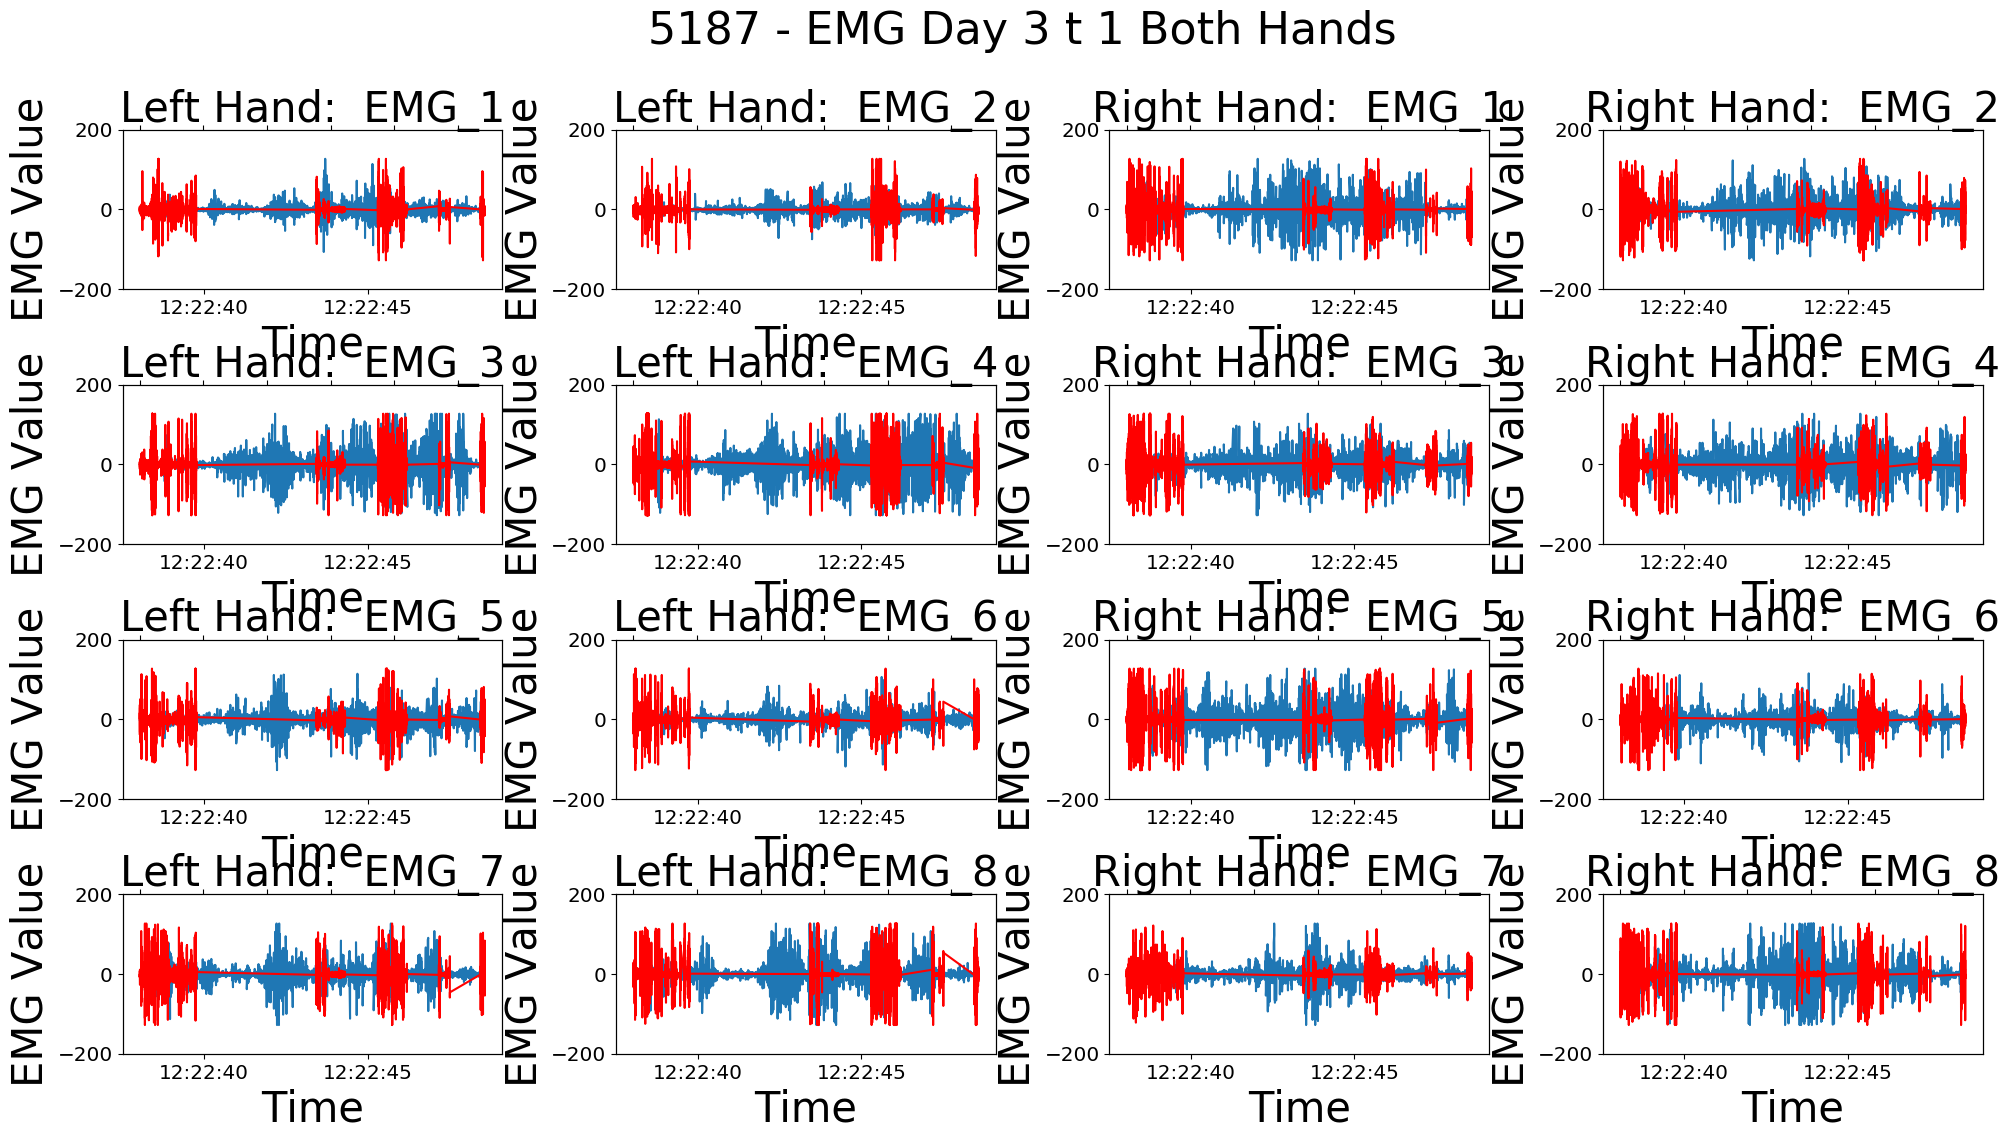
\includegraphics[width=\linewidth]{pictures/5187_EMG_Day3_t_1_average}
	\caption{Tourniquet EMG data with average in red}
	\label{fig:5187emgday3t1average}
\end{figure}

\subsection{Participant Generalizability Discussion}
\label{sec:Results:Generalizability:Discussion}

The combined dataset allowed the machine learning algorithms to train on several participants, each participant with different approaches to the procedures. The unique movements may all look similar, but the way participants grab and adjust tools can be different. 
The F1 score for the generalized population is close to the results generated for individual participants. The F1 score of the decision-tree algorithm for tying a tourniquet was on average 0.81 per participant and 0.74 across all participants. For wrapping a wound the F1 of the decision-tree algorithm was on average 0.90 per participant and 0.82 across all participants. Therefore, the algorithms are able to generalize across participants. The algorithms are also able to accurately detect a subset of procedures used inside an ambulance. While some procedures can be detected more accurately, others need improvements before the system can be deployed in real life scenarios.


\section{Discussion}
\label{sec:Results:Discussion}
The results clearly show that it is feasible to successfully recognize procedures performed by EMS personnel on patients using the Myo sensor. The results also show a high variance in accuracy depending on the algorithm and procedure. The comparison between the decision-tree, $k$-NN, SVM, and HMM algorithm highlight the strengths of the decision-tree algorithm. The algorithms were able to successfully detect the procedures both individually and over all participants.
\par $H_1$ hypothesized that CPR and Bag-valve-mask ventilation will have the highest accuracy for each machine learning algorithm, due to its unique movements. CPR and Bag-valve-mask ventilation had neither the highest F1 score for individual participants or for all participants. The result shows that more data preparation needs to take place in order to separate similar movements, such as dividing the procedures further into their task and training the algorithms on a task basis, while using the sequence of tasks to detect the procedure.
\par $H_2$ hypothesized that the recognition of a procedure through the sequence of fine-grained movements using a Hidden Markov Model will be more accurate than detection through training coarse-grained movement models. The HMM algorithm achieved the highest F1 score for Bag-Valve-Mask ventilation with the individual participants results. The overall participant generalizability placed the HMM algorithm third.
\par The F1 score for the HMM was expected to be significantly higher given its ability to detect data sequences. The results from training using individual participants and all participants show that the HMM placed second behind the decision-tree.
\par The F1 score of the SVM was lower than expected. Missing computing power for the large dataset resulted in limited ability to vary the parameters to improve the accuracy. 
\par The machine learning algorithms can be further improved by varying the parameters to a greater extent. The low performing SVM algorithm can be improved by varying the $gamma$ and $C$ value, and using a different kernel function.
\par The Hidden Markov Model algorithm can be further improved by optimizing selection of winners for all the models. Currently, the model with highest the log probability is picked as the correct result. The function can be improved by re-running the data, if the log probability of two models are withing a certain margin of error or printing out the probabilities to let the EMS personnel confirm the performed procedure after they return to their base.
\par Additionally, the Hidden Markov Model can be trained in a supervised manner. The hierarchical task analysis provides detail about the states included in a procedure. The states can be pre-defined and transition probabilities inferred. Furthermore, deep-learning algorithms, such as neural networks may achieve higher scores in case nonlinearity occurs in the dataset.
\par The generalizability can be further improved by collecting data from more participants. The data used in this thesis required participants to use specific hands for every procedure. Data, which includes left- and right-handed participants increases the generalizability.
\par The procedures represent those performed by EMS personnel on the way to the hospital inside of an ambulance. The movement of the ambulance introduces noise that can effect the accuracy of the machine learning algorithms. Future work can collect data in an ambulance simulation to improve real-life application.
\par Ambulances may include multiple EMS personnel, who can work on the patient simultaneously. The sensor has to be placed on all EMS personnel working on the patient in order to correctly identify the procedure. Future work can collect data from multiple participants at the same time and improve the machine learning algorithm to include data from more than two sensors.
\par Lastly, data from professionally trained EMS personnel may result in more consistent data, which may improve the score of all machine learning algorithms.
\par Overall, in order to use the technology in real world application, such as transmitting treatment information to a hospital in real-time requires a significantly higher detection accuracy. Unreliable treatment information can result in wrong preparation at the hospital, which may cause permanent injury or result in death. The procedure detection system needs to be further evaluated in real-life non-life threatening scenarios in order to obtain its effectiveness in improving communication between EMS personnel and hospital trauma staff. While there is room for improvement, the thesis is an initial step in detecting procedures inside of an ambulance.